\documentclass{beamer}
\usepackage{tikz,amsmath,hyperref,graphicx,stackrel,animate}
\usetikzlibrary{positioning,shadows,arrows,shapes,calc}
\newcommand{\argmax}{\operatornamewithlimits{argmax}}
\newcommand{\argmin}{\operatornamewithlimits{argmin}}
\mode<presentation>{\usetheme{Frankfurt}}
\DeclareMathOperator*{\softmax}{softmax}
\AtBeginSection[]
{
  \begin{frame}<beamer>
    \frametitle{Outline}
    \tableofcontents[currentsection,currentsubsection]
  \end{frame}
}
\title{Lecture 8: Nonlinearities}
\author{Mark Hasegawa-Johnson}
\date{ECE 417: Multimedia Signal Processing, Fall 2020}  
\begin{document}

% Title
\begin{frame}
  \maketitle
\end{frame}

% Title
\begin{frame}
  \tableofcontents
\end{frame}


%%%%%%%%%%%%%%%%%%%%%%%%%%%%%%%%%%%%%%%%%%%%
\section[Review]{Review: Neural Network}
\setcounter{subsection}{1}

\begin{frame}
  \frametitle{Review: How to train a neural network}
  \begin{enumerate}
  \item Find a {\bf training dataset} that contains $n$ examples showing the
    desired output, $\vec{y}_i$, that the NN should compute in
    response to input vector $\vec{x}_i$:
    \[
    {\mathcal D}=\left\{(\vec{x}_1,\vec{y}_1),\ldots,(\vec{x}_n,\vec{y}_n)\right\}
    \]
    \item Randomly {\bf initialize} the weights and biases, $W^{(1)}$,
      $\vec{b}^{(1)}$, $W^{(2)}$, and $\vec{b}^{(2)}$.
    \item Perform {\bf forward propagation}: find out what the neural
      net computes as $\hat{y}_i$ for each $\vec{x}_i$.
    \item Define a {\bf loss function} that measures
      how badly $\hat{y}$ differs from $\vec{y}$.
    \item Perform {\bf back propagation} to improve $W^{(1)}$,
      $\vec{b}^{(1)}$, $W^{(2)}$, and $\vec{b}^{(2)}$.
    \item Repeat steps 3-5 until convergence.
  \end{enumerate}
\end{frame}

\begin{frame}
  \frametitle{Review: Second Layer = Piece-Wise Approximation}

  The second layer of the network approximates $\hat{y}$ using a bias term $\vec{b}$,
  plus correction vectors $\vec{w}_j^{(2)}$, each scaled by its activation $h_j$:
  \[
  \hat{y} = \vec{b}^{(2)} + \sum_j \vec{w}_{j}^{(2)} h_j
  \]
  The activation, $h_j$, is a number between 0 and 1.  For example, we could
  use the logistic sigmoid function:
  \[
  h_k = \sigma\left(e_k^{(1)}\right)=\frac{1}{1+\exp(-e_k^{(1)})}\in\left(0,1\right)
  \]
  The logistic sigmoid is a differentiable approximation to a unit step function.
\end{frame}

\begin{frame}
  \frametitle{Review: First Layer = A Series of Decisions}

  The first layer of the network decides whether or not to ``turn on'' each of the
  $h_j$'s.  It does this by comparing $\vec{x}$ to a series of linear threshold vectors:
  \[
  h_k = \sigma\left(\bar{w}_k^{(1)}\vec{x}\right)\approx\begin{cases}
  1 & \bar{w}_k^{(1)}\vec{x} > 0\\
  0 & \bar{w}_k^{(1)}\vec{x} < 0
  \end{cases}
  \]
\end{frame}

\begin{frame}
  \frametitle{Gradient Descent: How do we improve $W$ and $b$?}  Given
  some initial neural net parameter (called $u_{kj}$ in this figure),
  we want to find a better value of the same parameter.  We do that
  using gradient descent:
  \[
  u_{kj} \leftarrow u_{kj}-\eta\frac{d{\mathcal L}}{du_{kj}},
  \]
  where $\eta$ is a learning rate (some small constant, e.g., $\eta=0.02$ or so).
  \centerline{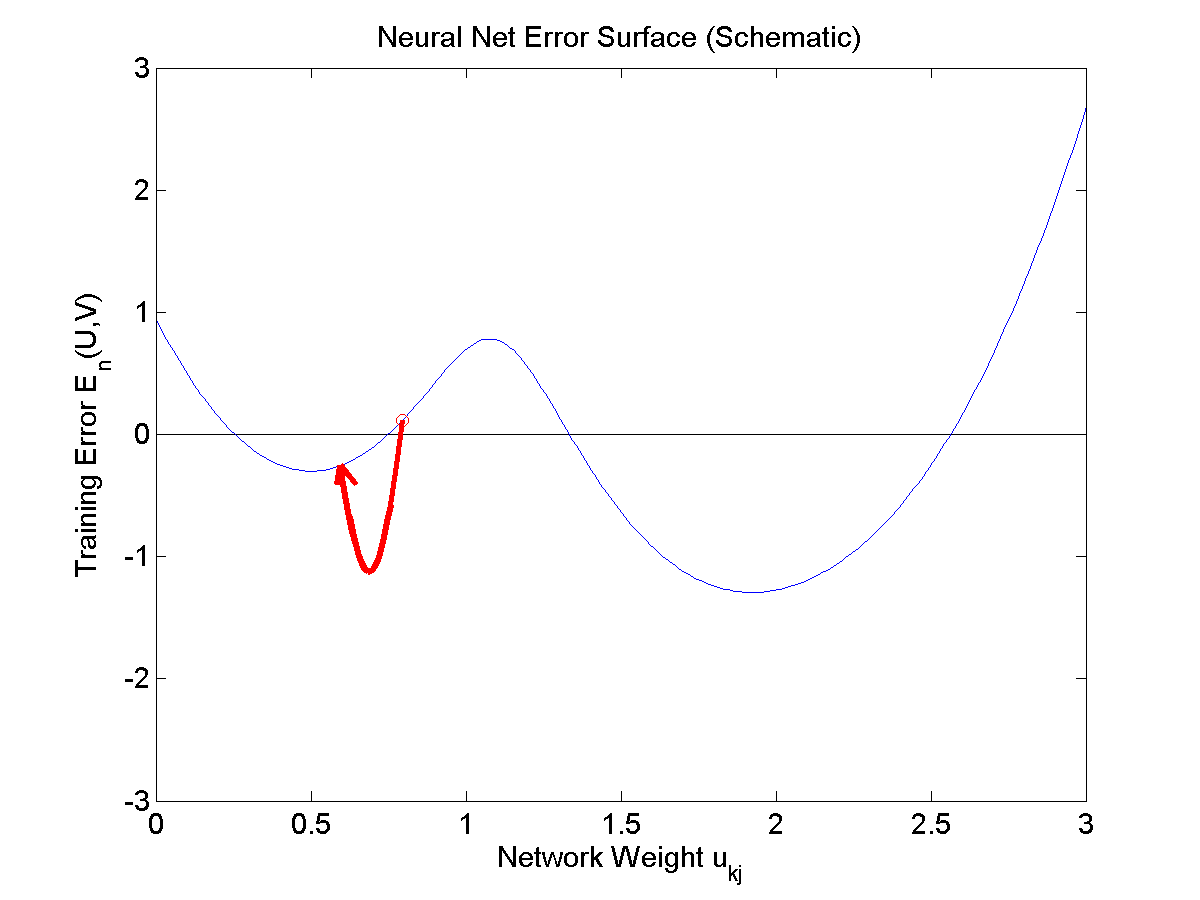
\includegraphics[width=2in]{../lec07/figs/nn_errorsurf1.png}}
\end{frame}

%%%%%%%%%%%%%%%%%%%%%%%%%%%%%%%%%%%%%%%%%%%%
\section{Binary Nonlinearities}
\setcounter{subsection}{1}

\begin{frame}
  \begin{columns}[t]
    \column{1.85in}
    \begin{block}{The Basic Binary  Nonlinearity: Unit Step (a.k.a. Heaviside function)}
      \[
      u\left(\bar{w}_k^{(1)}\vec{x}\right)=\begin{cases}
      1 & \bar{w}_k^{(1)}\vec{x} > 0\\
      0 & \bar{w}_k^{(1)}\vec{x} < 0
      \end{cases}
      \]
      \centerline{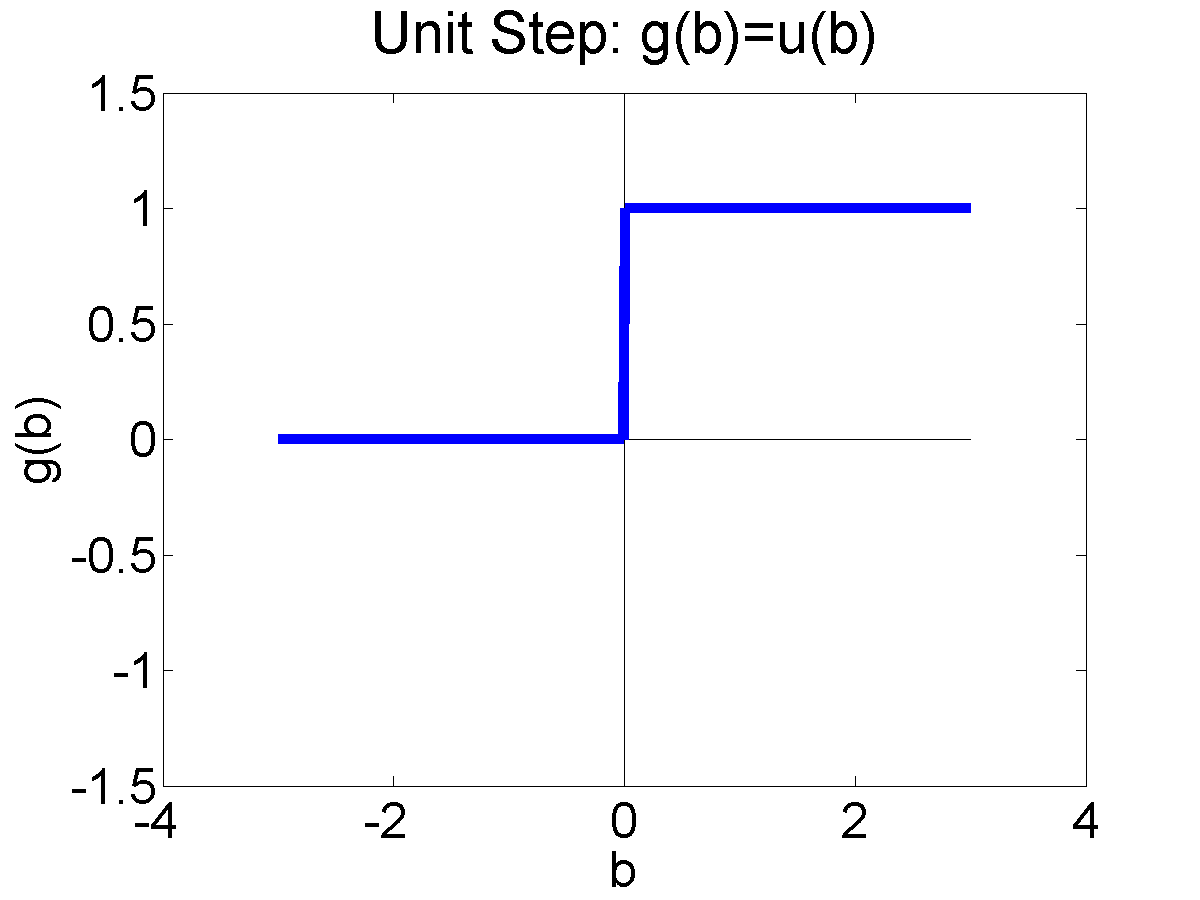
\includegraphics[width=1.75in]{../lec07/figs/nn_unitstep.png}}
    \end{block}
    \column{2.65in}
    \begin{block}{Pros and Cons of the Unit Step}
      \begin{itemize}
      \item {\bf Pro:} it gives exactly piece-wise constant
        approximation of any desired $\vec{y}$.
      \item {\bf Con:} if $h_k=u(e_k)$, then you can't use
        back-propagation to train the neural network.
      \end{itemize}
      Remember back-prop:
      \[
      \frac{d{\mathcal L}}{dw_{kj}}=
      \sum_k\left(\frac{d{\mathcal L}}{dh_k}\right)
      \left(\frac{\partial h_k}{\partial e_k}\right)
      \left(\frac{\partial e_k}{\partial w_{kj}}\right)
      \]
      but $du(x)/dx$ is a Dirac delta function ---
      zero everywhere, except where it's infinite.
    \end{block}
  \end{columns}
\end{frame}
  
\begin{frame}
  \begin{columns}[t]
    \column{2.25in}
    \begin{block}{The Differentiable Approximation: Logistic Sigmoid}
      \[
      \sigma(b)=\frac{1}{1+e^{-b}}
      \]
      \centerline{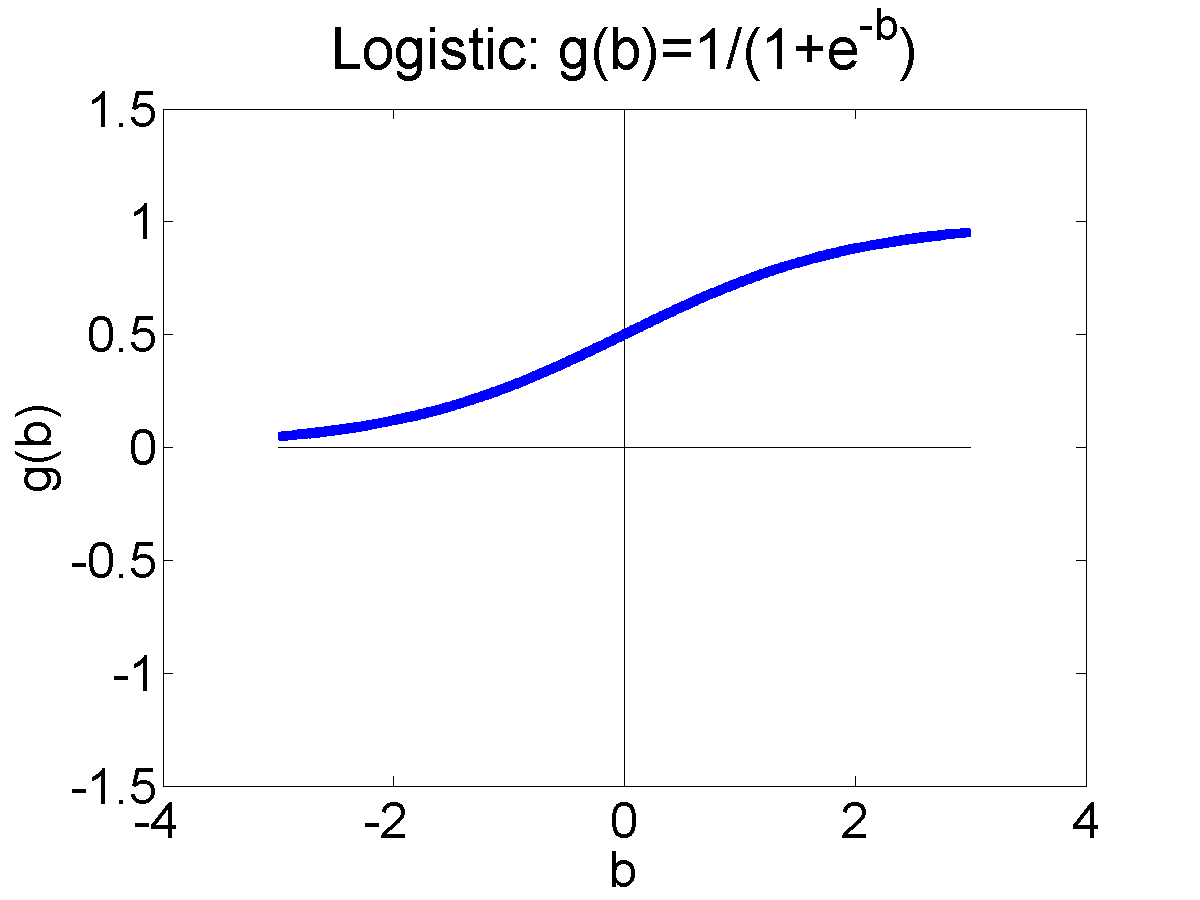
\includegraphics[width=1.75in]{../lec07/figs/nn_logistic.png}}
    \end{block}
    \column{2.25in}
    \begin{block}{Why to use the logistic function}
      \[
      \sigma(b) = \begin{cases}
        1 & b\rightarrow\infty\\
        0 & b\rightarrow -\infty\\
        \mbox{in between} & \mbox{in between}
      \end{cases}
      \]
      and $\sigma(b)$ is smoothly differentiable, so
      back-prop works.
    \end{block}
  \end{columns}
\end{frame}

\begin{frame}
  \frametitle{Derivative of a sigmoid}
  The derivative of a sigmoid is pretty easy to calculate:
  \[
  \sigma(x)=\frac{1}{1+e^{-x}},~~~\frac{d\sigma}{dx}=\frac{e^{-x}}{(1+e^{-x})^2}
  \]
  An interesting fact that's extremely useful, in computing back-prop,
  is that if $h=\sigma(x)$, then we can write the derivative in terms
  of $h$, without any need to store $x$:
  \begin{align*}
    \frac{d\sigma}{dx} &=\frac{e^{-x}}{(1+e^{-x})^2}\\
    &=\left(\frac{1}{1+e^{-x}}\right)\left(\frac{e^{-x}}{1+e^{-x}}\right)\\
    &=\left(\frac{1}{1+e^{-x}}\right)\left(1-\frac{1}{1+e^{-x}}\right)\\
    &=\sigma(x)(1-\sigma(x))\\
    &=h(1-h)\\
  \end{align*}
\end{frame}

\begin{frame}
  \begin{columns}[t]
    \column{2.25in}
    \begin{block}{Step function and its derivative}
      \centerline{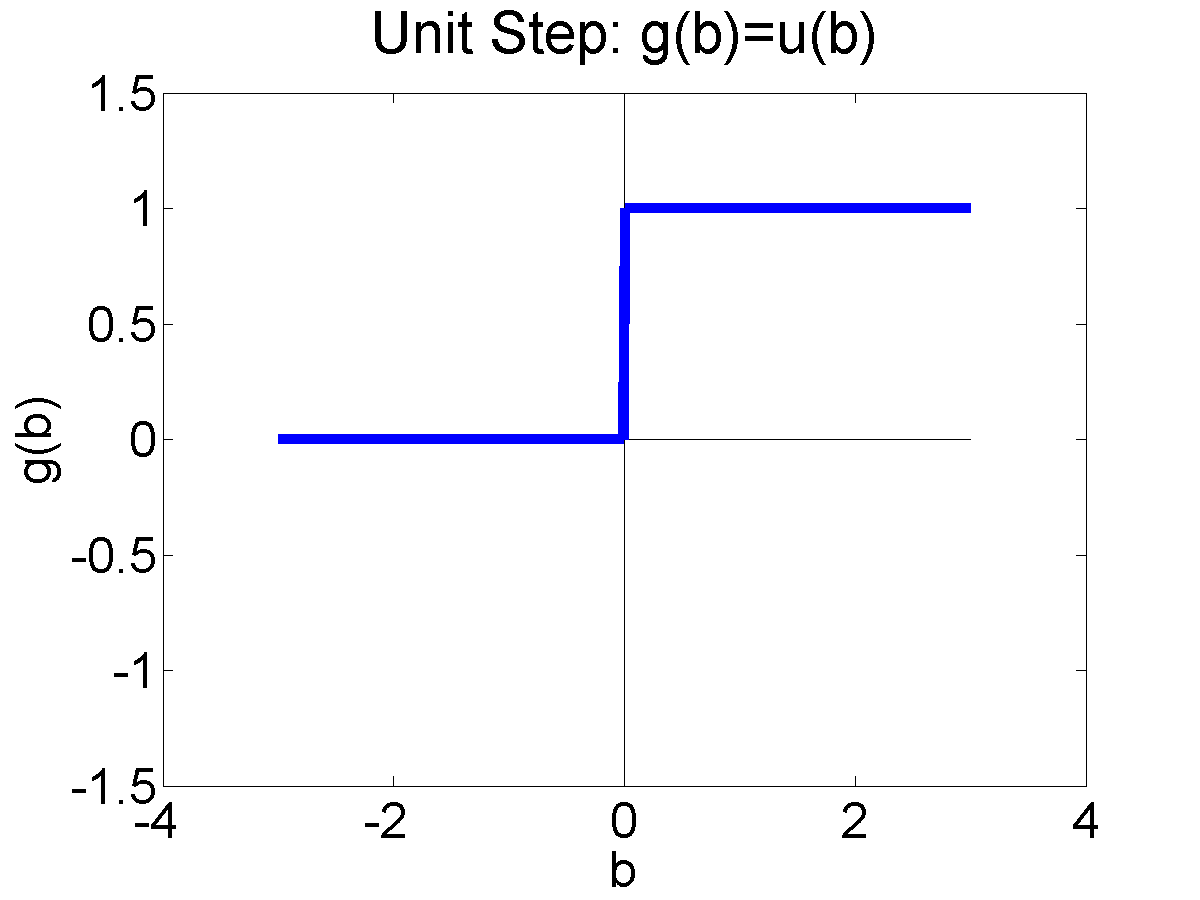
\includegraphics[width=1.75in]{../lec07/figs/nn_unitstep.png}}
      \begin{itemize}
      \item The derivative of the step function is the Dirac
        delta, which is not very useful in backprop.
      \end{itemize}
    \end{block}
    \column{2.25in}
    \begin{block}{Logistic function and its derivative}
      \centerline{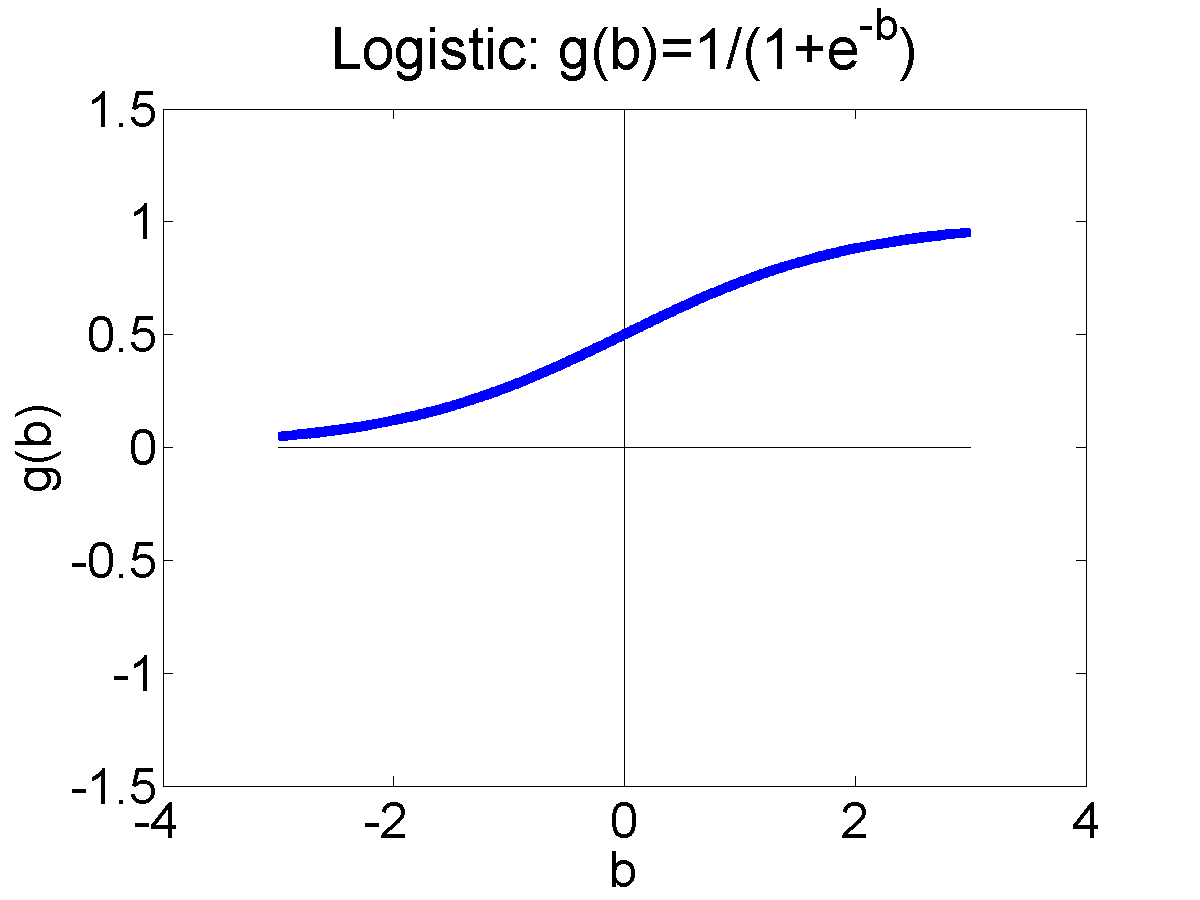
\includegraphics[width=1.75in]{../lec07/figs/nn_logistic.png}}
      \centerline{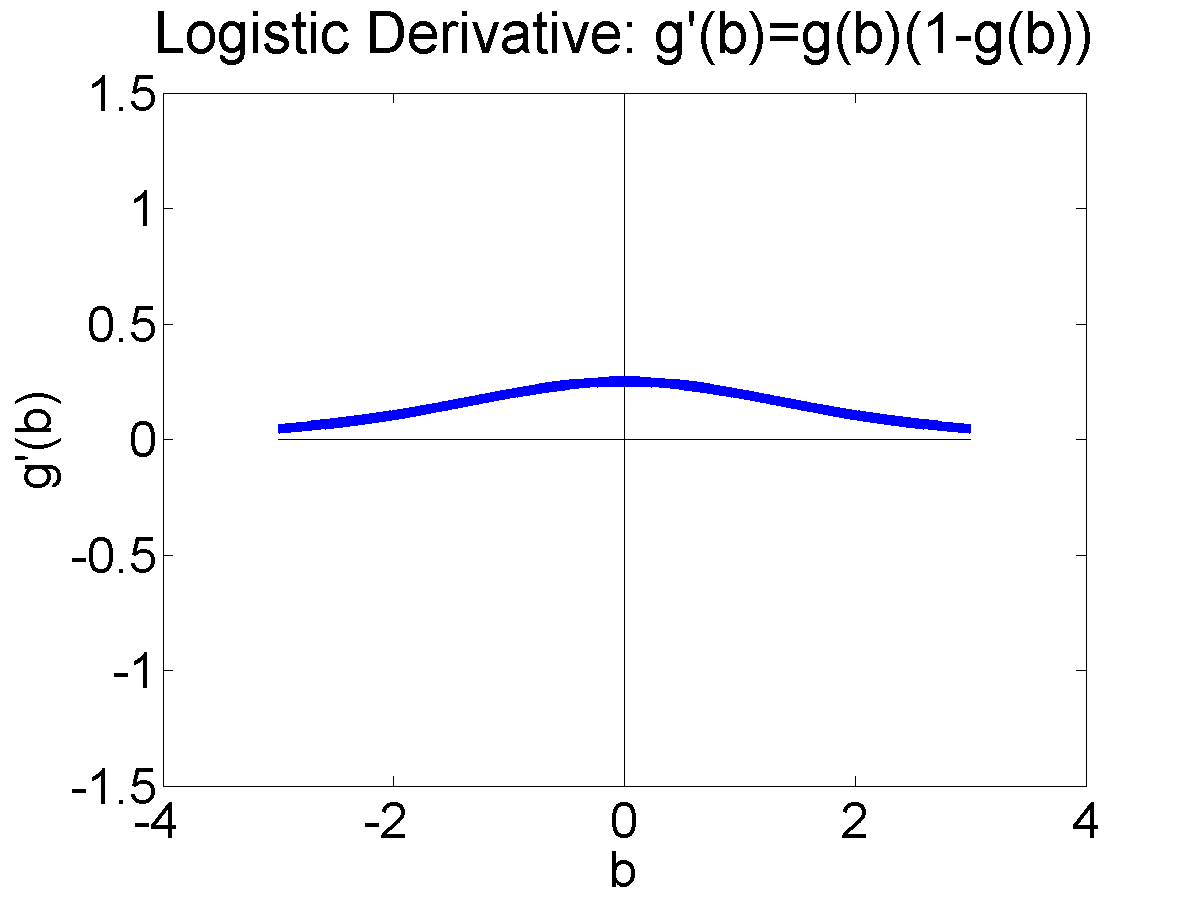
\includegraphics[width=1.75in]{../lec07/figs/nn_logisticprime.png}}
    \end{block}
  \end{columns}
\end{frame}

\begin{frame}
  \frametitle{Signum and Tanh}

  The signum function is a signed binary nonlinearity.  It is used if,
  for some reason, you want your output to be
  $h\in\left\{-1,1\right\}$, instead of $h\in\left\{0,1\right\}$:
  \[
  \mbox{sign}(b)=\begin{cases}
  -1 & b<0\\
  1 & b>0
  \end{cases}
  \]
  It is usually approximated by the hyperbolic tangent function
  (tanh), which is just a scaled shifted version of the sigmoid:
  \begin{displaymath}
    \tanh(b) = \frac{e^b-e^{-b}}{e^b+e^{-b}}
    = \frac{1-e^{-2b}}{1+e^{-2b}}
    = 2\sigma(2b)-1
  \end{displaymath}
  and which has a scaled version of the sigmoid derivative:
  \begin{align*}
    \frac{d\tanh(b)}{db} =\left(1-\tanh^2(b)\right)
  \end{align*}
\end{frame}

\begin{frame}
  \begin{columns}[t]
    \column{2.25in}
    \begin{block}{Signum function and its derivative}
      \centerline{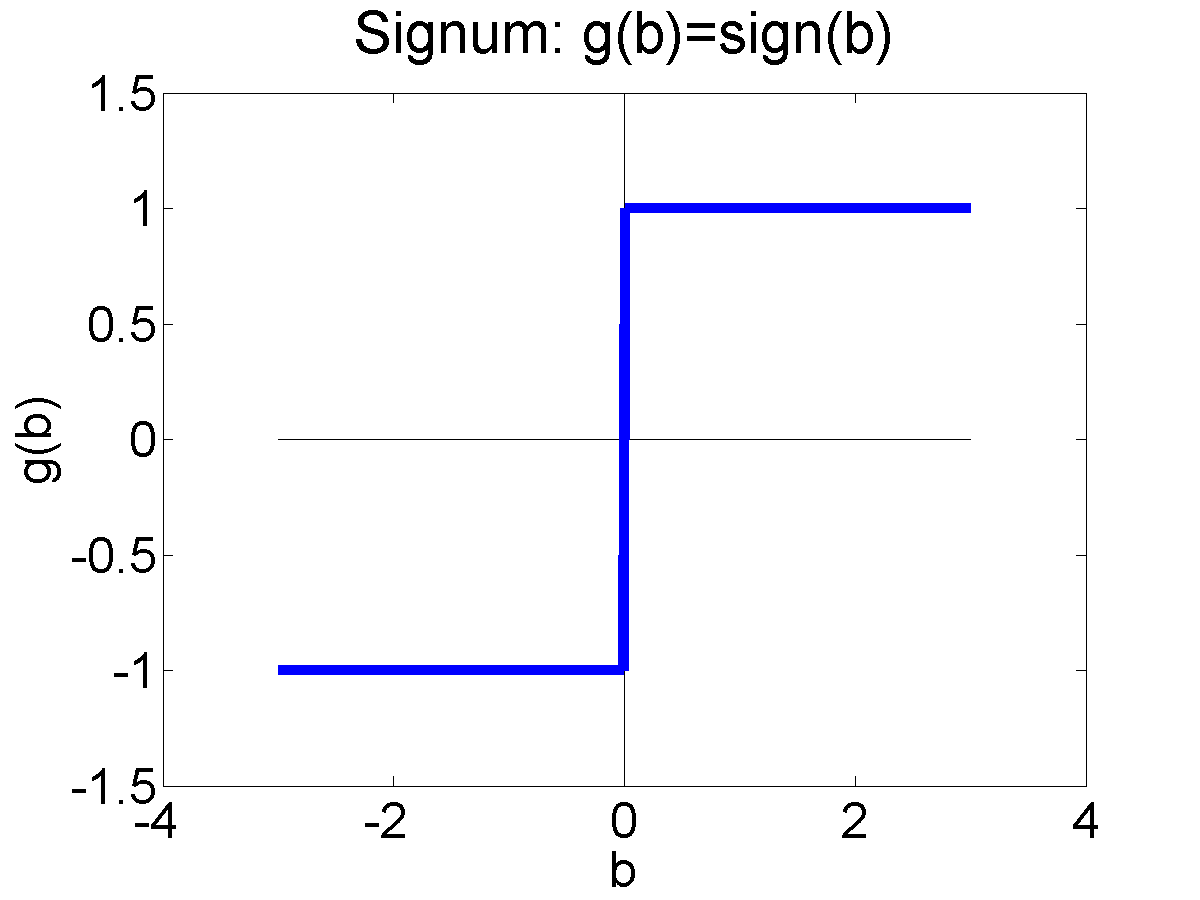
\includegraphics[width=1.75in]{../lec07/figs/nn_signum.png}}
      \begin{itemize}
      \item The derivative of the signum function is the Dirac
        delta, which is not very useful in backprop.
      \end{itemize}
    \end{block}
    \column{2.25in}
    \begin{block}{Tanh function and its derivative}
      \centerline{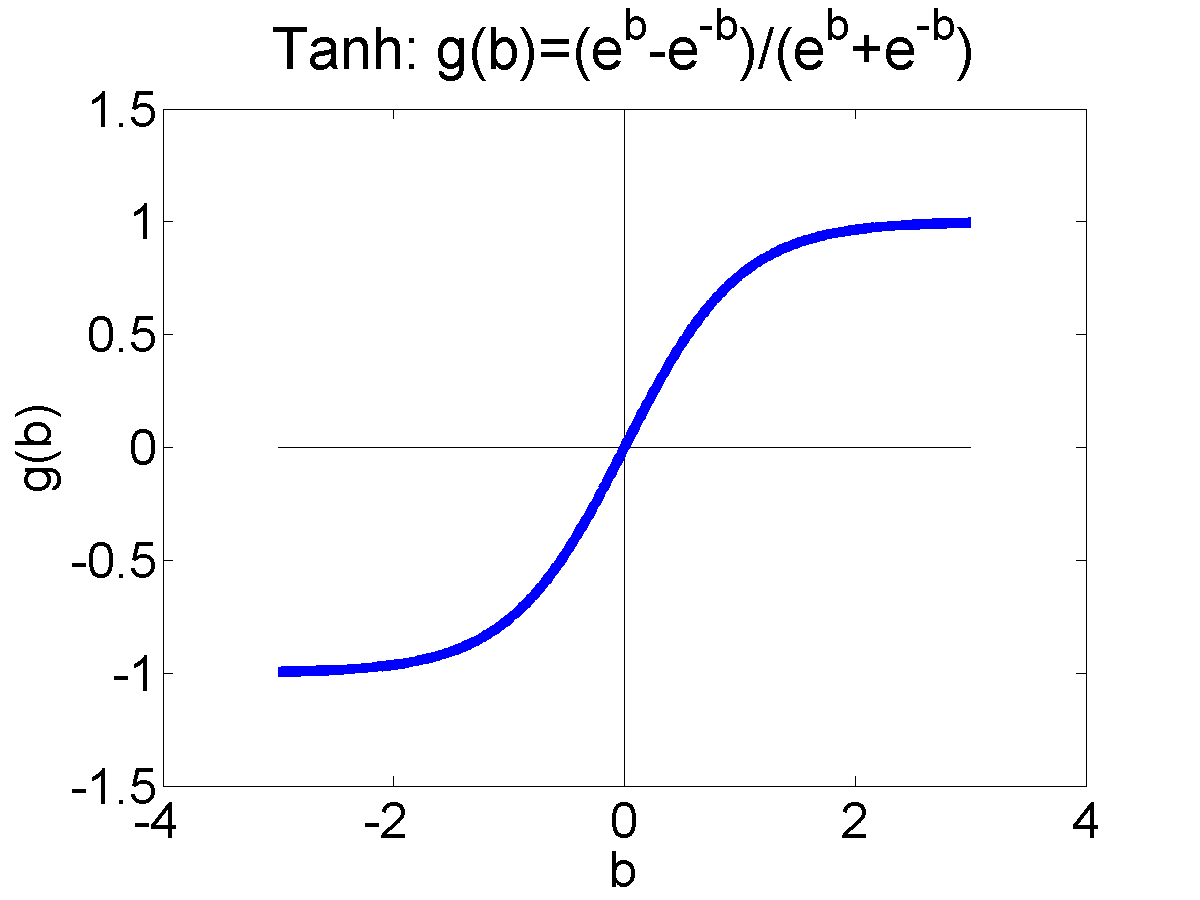
\includegraphics[width=1.75in]{../lec07/figs/nn_tanh.png}}
      \centerline{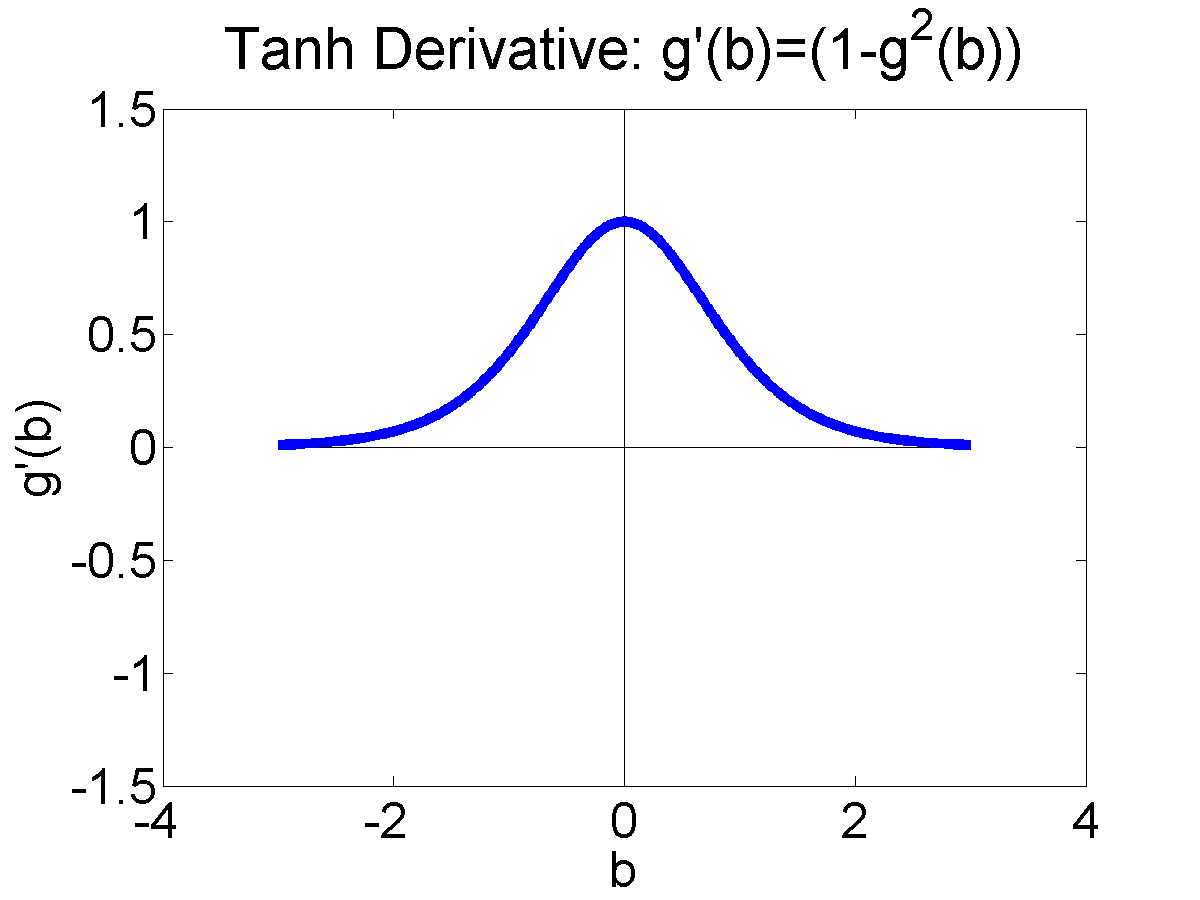
\includegraphics[width=1.75in]{../lec07/figs/nn_tanhprime.png}}
    \end{block}
  \end{columns}
\end{frame}

\begin{frame}
  \frametitle{A suprising problem with the sigmoid: Vanishing gradients}
  \centerline{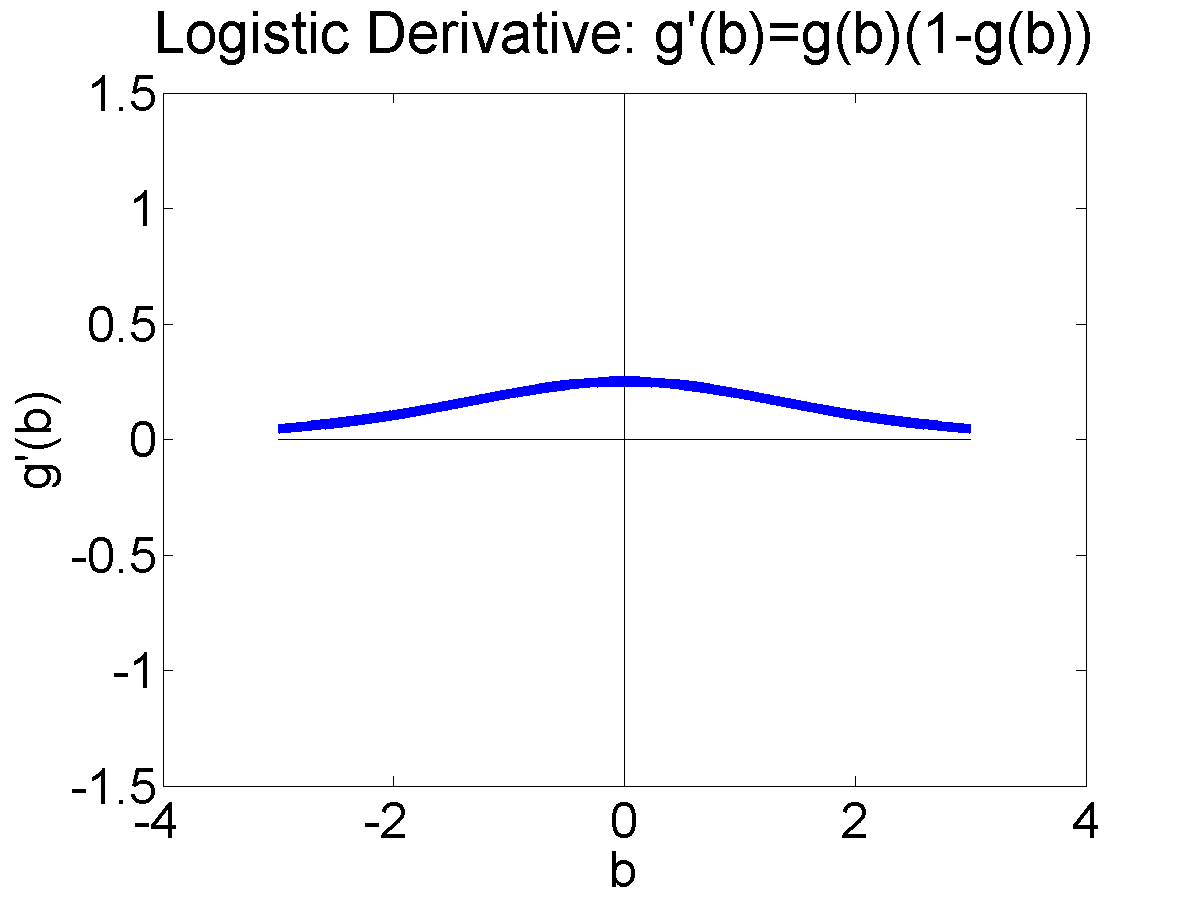
\includegraphics[width=1in]{../lec07/figs/nn_logisticprime.png}}
  
  The sigmoid has a surprising problem: for large values of $w$,
  $\sigma'(wx)\rightarrow 0$.
  \begin{itemize}
  \item When we begin training, we start with small values of $w$.
    $\sigma'(wx)$ is reasonably large, and training proceeds.
  \item If $w$ and $\nabla_{w}{\mathcal L}$ are vectors in opposite
    directions, then $w\rightarrow w-\eta\nabla_{w}{\mathcal L}$ makes
    $w$ larger.  After a few iterations, $w$ gets very large.  At that
    point, $\sigma'(wx)\rightarrow 0$, and training effectively stops.
  \item After that point, even if the neural net sees new training
    data that don't match what it has already learned, it can no
    longer change.  We say that it has suffered from the ``vanishing
    gradient problem.''
  \end{itemize}
\end{frame}
    
\begin{frame}
  \frametitle{A solution to the vanishing gradient problem: ReLU}
  \centerline{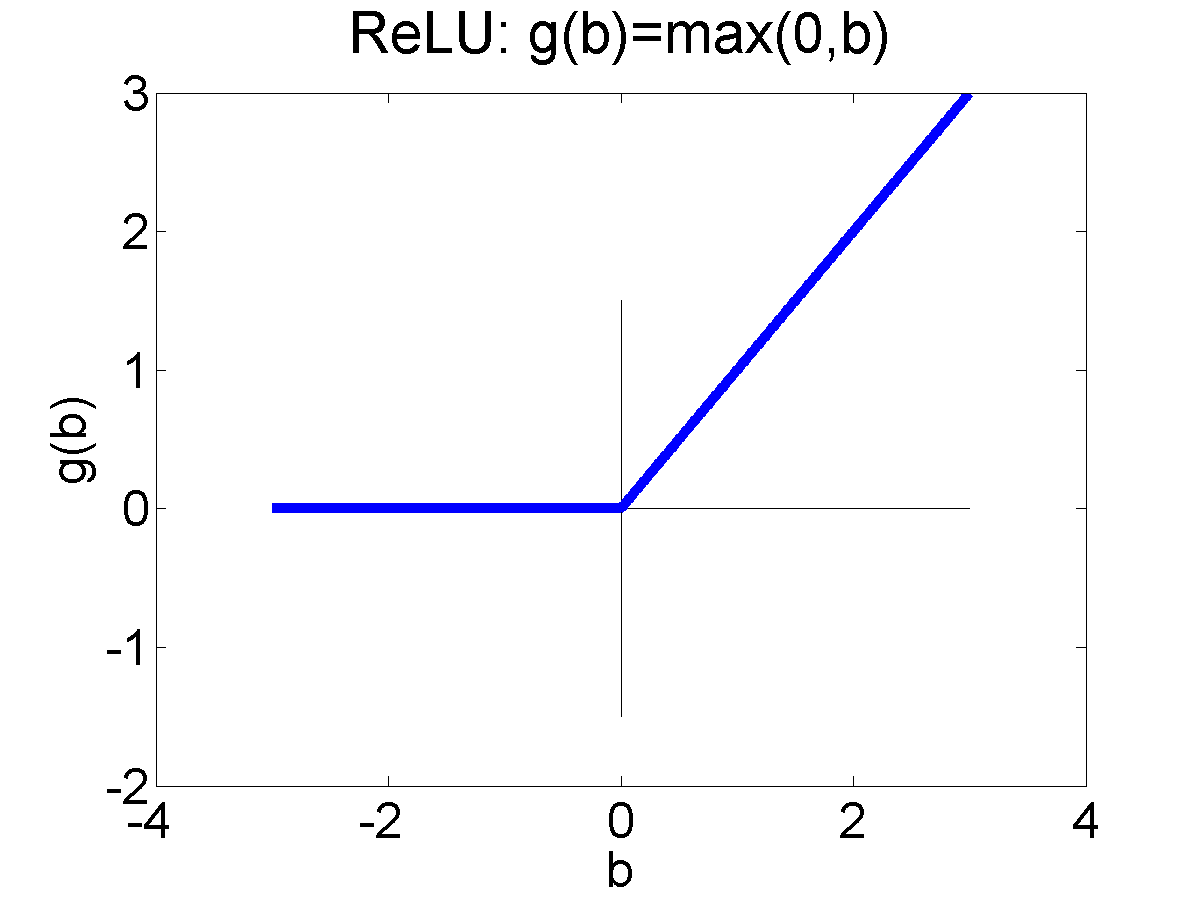
\includegraphics[width=1in]{../lec07/figs/nn_relu.png}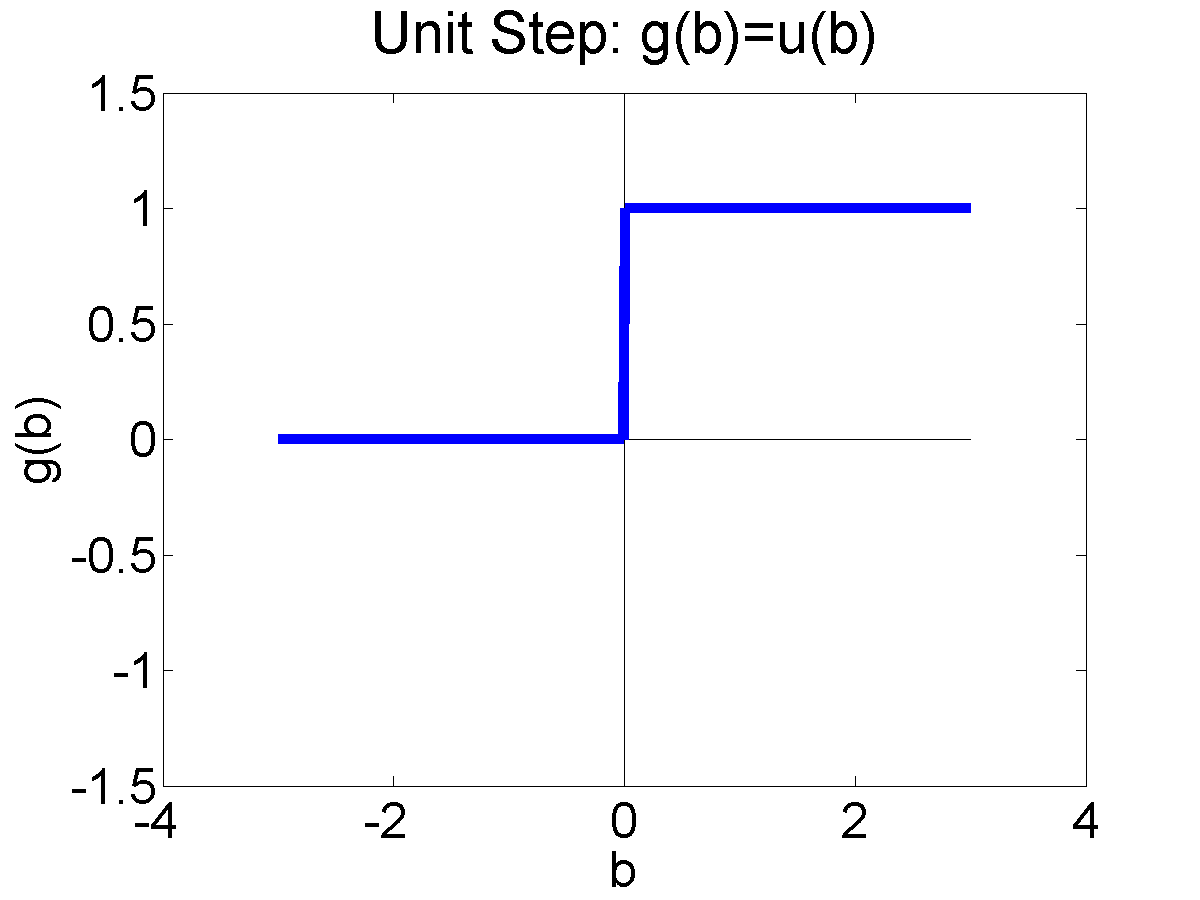
\includegraphics[width=1in]{../lec07/figs/nn_unitstep.png}}

  The most ubiquitous solution to the vanishing gradient problem is to
  use a ReLU (rectified linear unit) instead of a sigmoid.  The ReLU
  is given by
  \[
  \mbox{ReLU}(b) = \begin{cases}
    b & b\ge 0\\
    0 & b\le 0,
  \end{cases}
  \]
  and its derivative is the unit step.  Notice that the
  unit step is equally large ($u(wx)=1$)  for any positive value ($wx>0$), so
  no matter how large $w$ gets, back-propagation continues to work.
\end{frame}

\begin{frame}
  \frametitle{A solution to the vanishing gradient problem: ReLU}
  \centerline{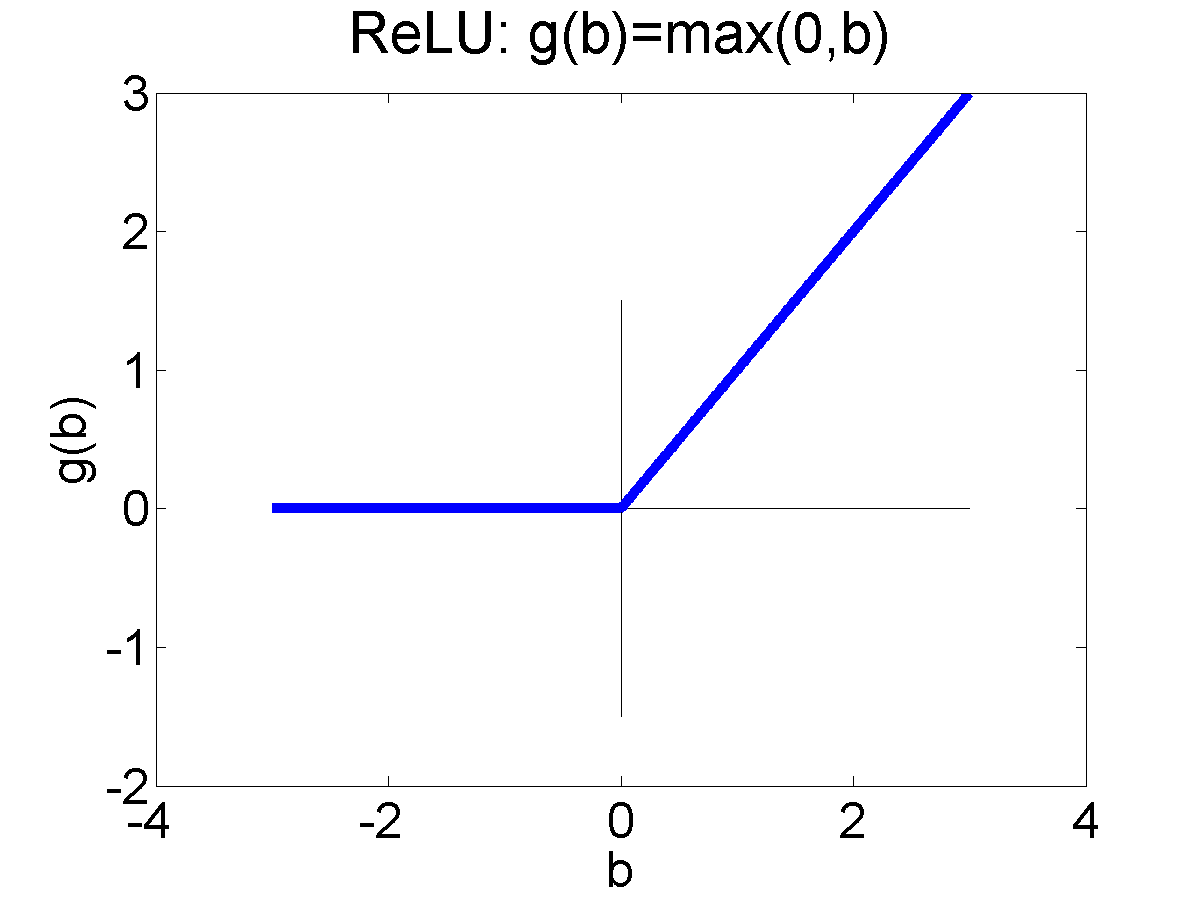
\includegraphics[width=1in]{../lec07/figs/nn_relu.png}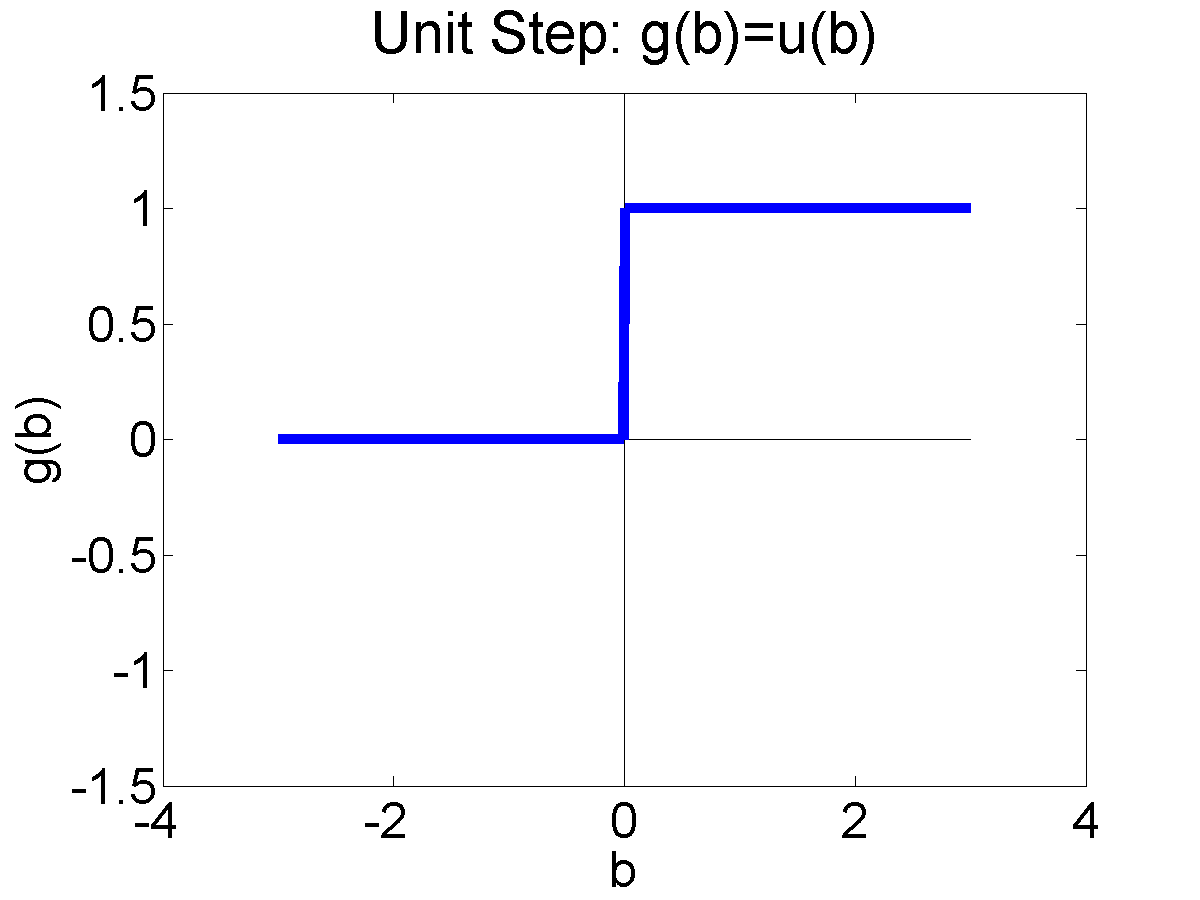
\includegraphics[width=1in]{../lec07/figs/nn_unitstep.png}}

  \begin{itemize}
    \item {\bf Pro:} The ReLU derivative is equally large
      ($\frac{d\mbox{ReLU}(wx)}{d(wx)}=1$) for any positive value
      ($wx>0$), so no matter how large $w$ gets, back-propagation
      continues to work.
    \item {\bf Con:} If the ReLU is used as a hidden unit
      ($h_j=\mbox{ReLU}(e_j)$), then your output is no longer a
      piece-wise constant approximation of $\vec{y}$.  It is now
      piece-wise linear.
    \item On the other hand, maybe piece-wise linear is
      better than piece-wise constant, so\ldots
  \end{itemize}
\end{frame}
      
\begin{frame}
  \frametitle{A solution to the vanishing gradient problem: the ReLU}
  \centerline{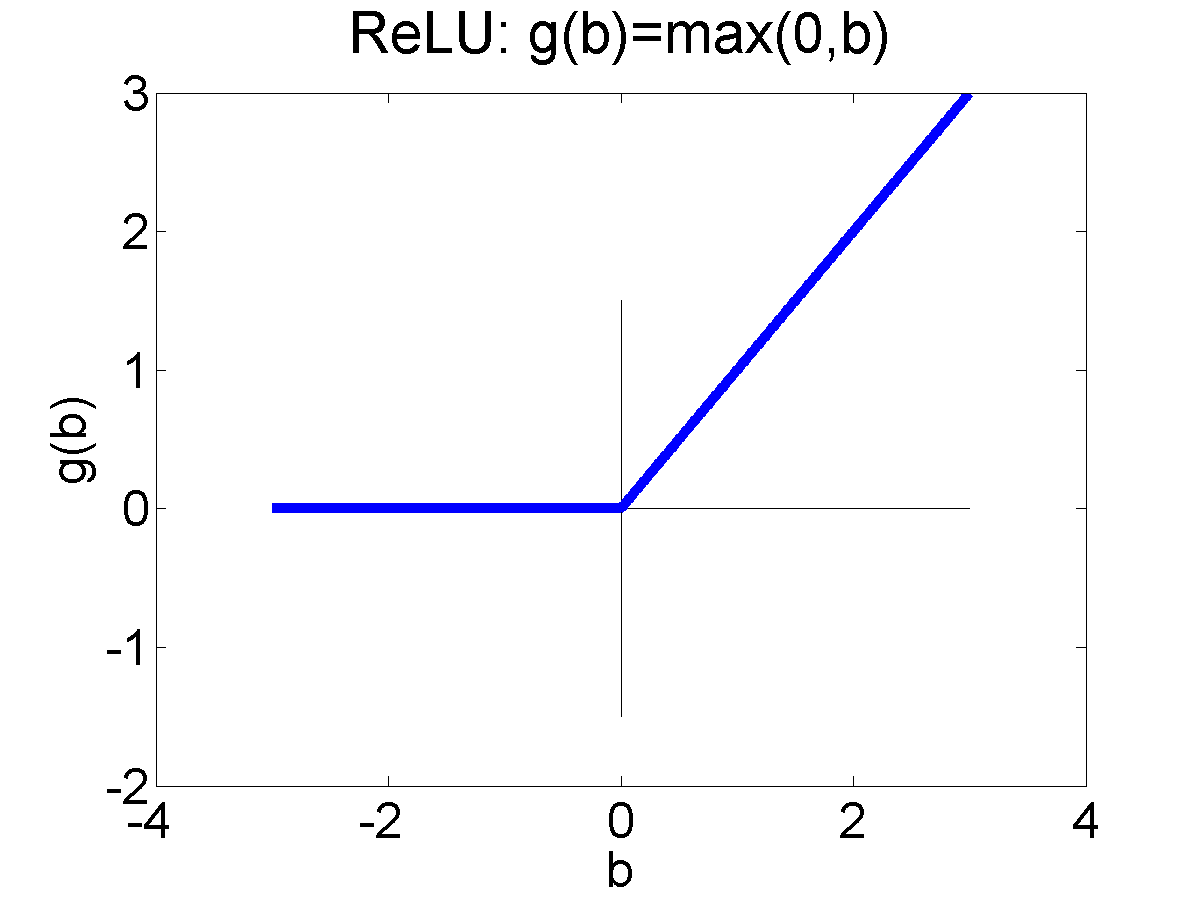
\includegraphics[width=1in]{../lec07/figs/nn_relu.png}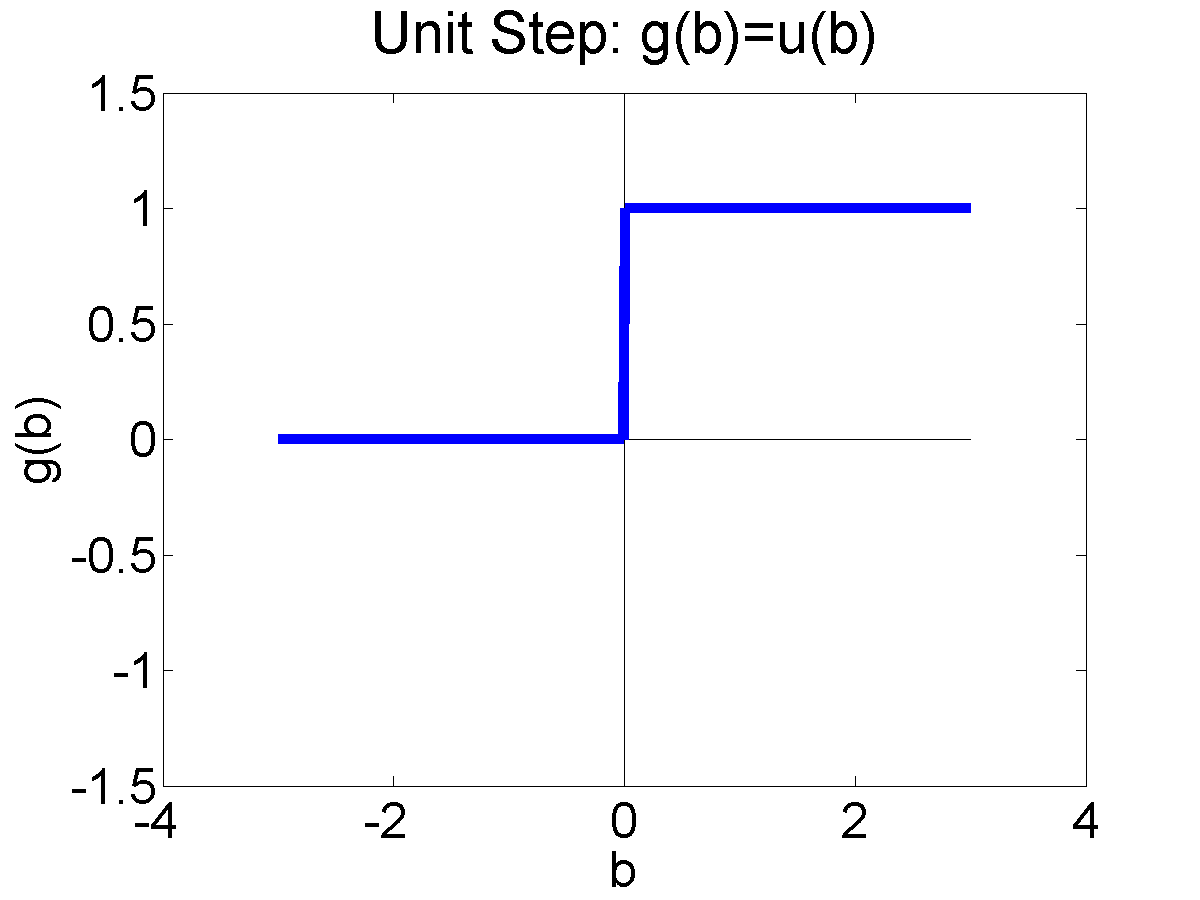
\includegraphics[width=1in]{../lec07/figs/nn_unitstep.png}}

  \begin{itemize}
    \item {\bf Pro:} The ReLU derivative is equally large
      ($\frac{d\mbox{ReLU}(wx)}{d(wx)}=1$) for any positive value
      ($wx>0$), so no matter how large $w$ gets, back-propagation
      continues to work.
    \item {\bf Pro:} If the ReLU is used as a hidden unit
      ($h_j=\mbox{ReLU}(e_j)$), then your output is no longer a
      piece-wise constant approximation of $\vec{y}$.  It is now
      piece-wise linear.
    \item {\bf Con:} ??
  \end{itemize}
\end{frame}

\begin{frame}
  \frametitle{The dying ReLU problem}
  \centerline{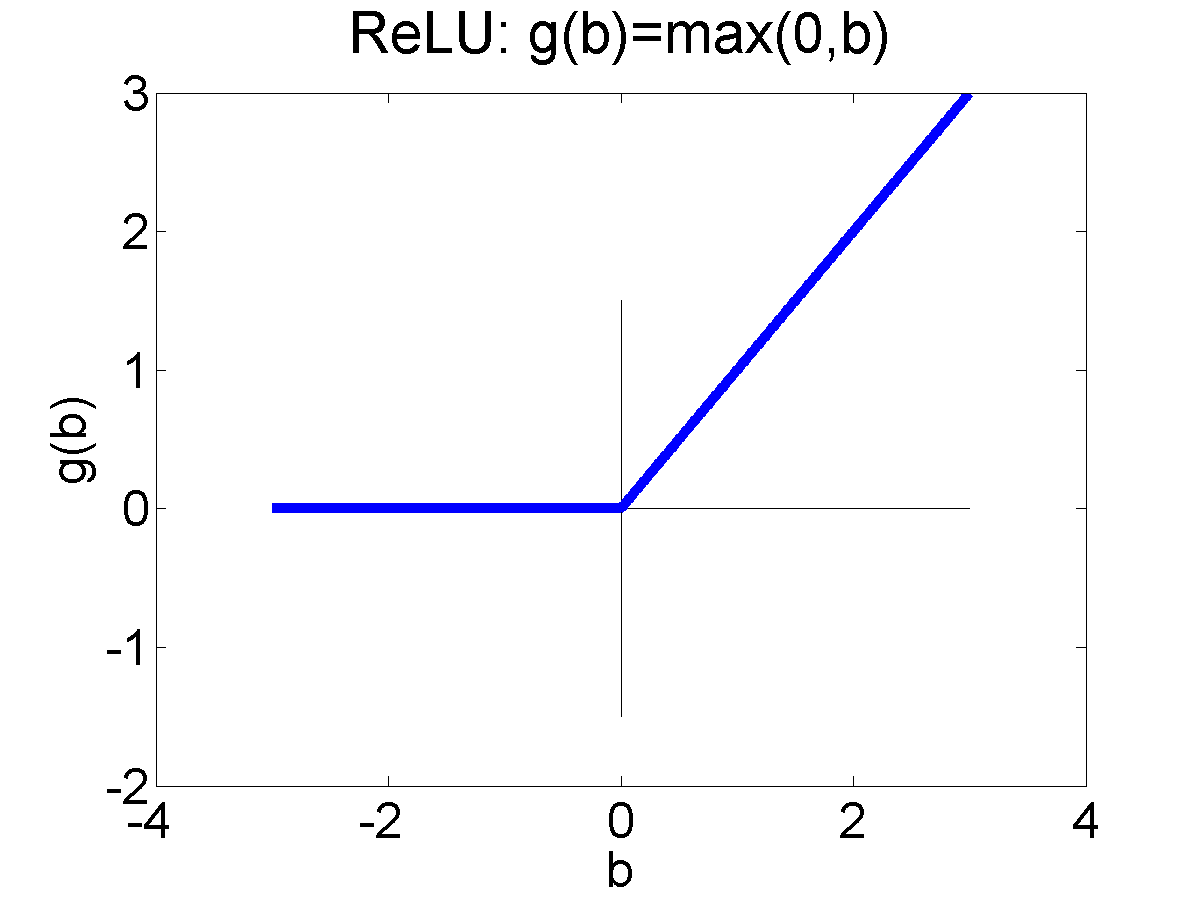
\includegraphics[width=1in]{../lec07/figs/nn_relu.png}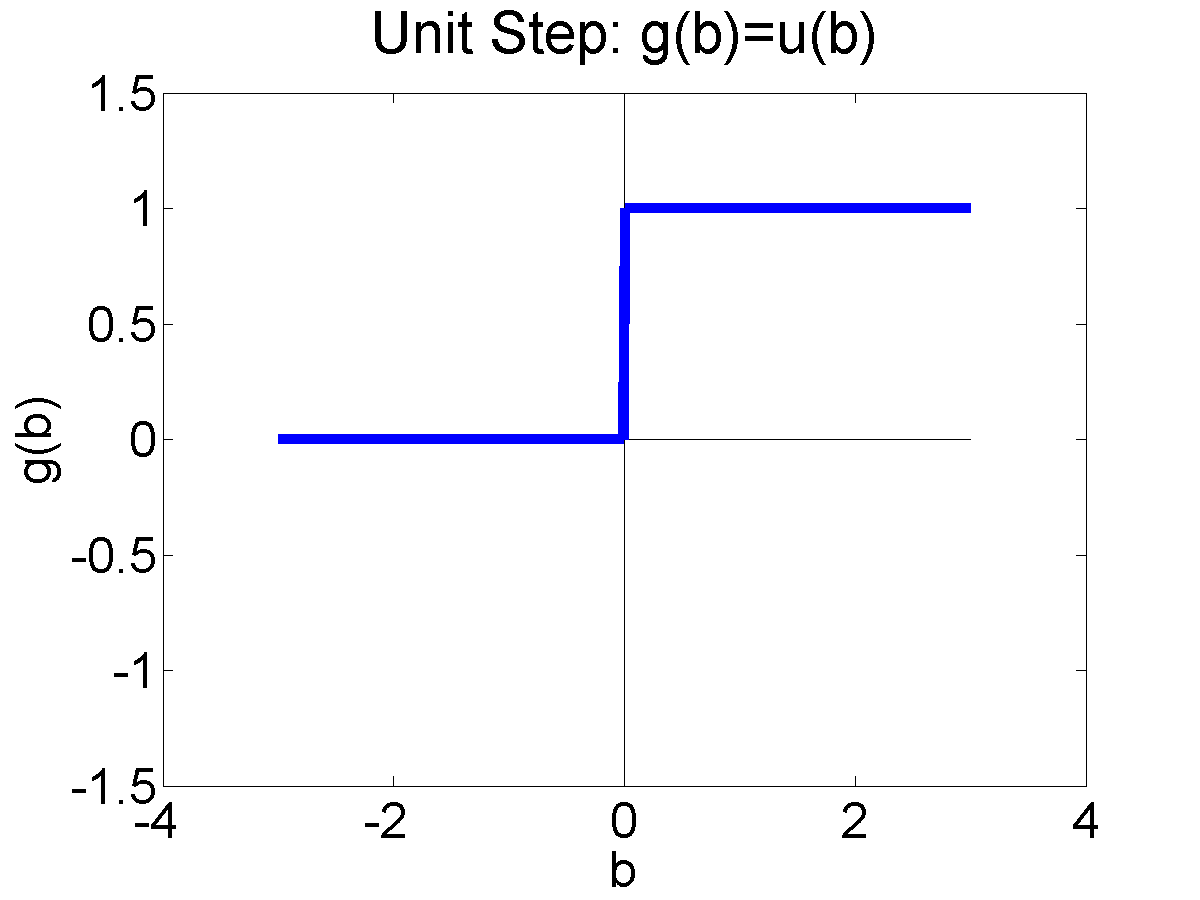
\includegraphics[width=1in]{../lec07/figs/nn_unitstep.png}}

  \begin{itemize}
    \item {\bf Pro:} The ReLU derivative is equally large
      ($\frac{d\mbox{ReLU}(wx)}{d(wx)}=1$) for any positive value
      ($wx>0$), so no matter how large $w$ gets, back-propagation
      continues to work.
    \item {\bf Pro:} If the ReLU is used as a hidden unit
      ($h_j=\mbox{ReLU}(e_j)$), then your output is no longer a
      piece-wise constant approximation of $\vec{y}$.  It is now
      piece-wise linear.
    \item {\bf Con:} If $wx+b<0$, then
      ($\frac{d\mbox{ReLU}(wx)}{d(wx)}=0$), and learning stops.
      In the worst case, if $b$ becomes very negative, then all of the
      hidden nodes are turned off---the network computes nothing, and
      no learning can take place!  This is called the ``Dying ReLU
      problem.''
  \end{itemize}
\end{frame}

\begin{frame}
  \frametitle{Solutions to the Dying ReLU problem}

  \begin{itemize}
  \item {\bf Softplus:}  Pro: always positive.  Con: gradient$\rightarrow 0$ as $x\rightarrow -\infty$.
    \[
    f(x) = \ln\left(1+e^x\right)
    \]
  \item {\bf Leaky ReLU:} Pro: gradient constant, output piece-wise linear.  Con:
    negative part might fail to match your dataset.
    \[
    f(x) = \begin{cases}
      x & x \ge 0\\
      0.01x & x \le 0
    \end{cases}
    \]
  \item {\bf Parametric ReLU (PReLU:)} Pro: gradient constant, ouput
    PWL.  The slope of the negative part ($a$) is a trainable
    parameter, so can adapt to your dataset.  Con: you have to train it.
    \[
    f(x) = \begin{cases}
      x & x \ge 0\\
      ax & x \le 0
    \end{cases}
    \]
  \end{itemize}
\end{frame}

%%%%%%%%%%%%%%%%%%%%%%%%%%%%%%%%%%%%%%%%%%%%%%%%%%%%%%%%%%%%%%%
\section[Classifiers]{Classifiers}
\setcounter{subsection}{1}

\begin{frame}
  \frametitle{A classifier target funtion}

  A ``classifier'' is a neural network with discrete ouputs.  For
  example, suppose you need to color a 2D picture.  The goal is to
  output $\hat{y}(\vec{x})=1$ if $\vec{x}$ should be red, and
  $\hat{y}=-1$ if $\vec{x}$ should be blue:

  \centerline{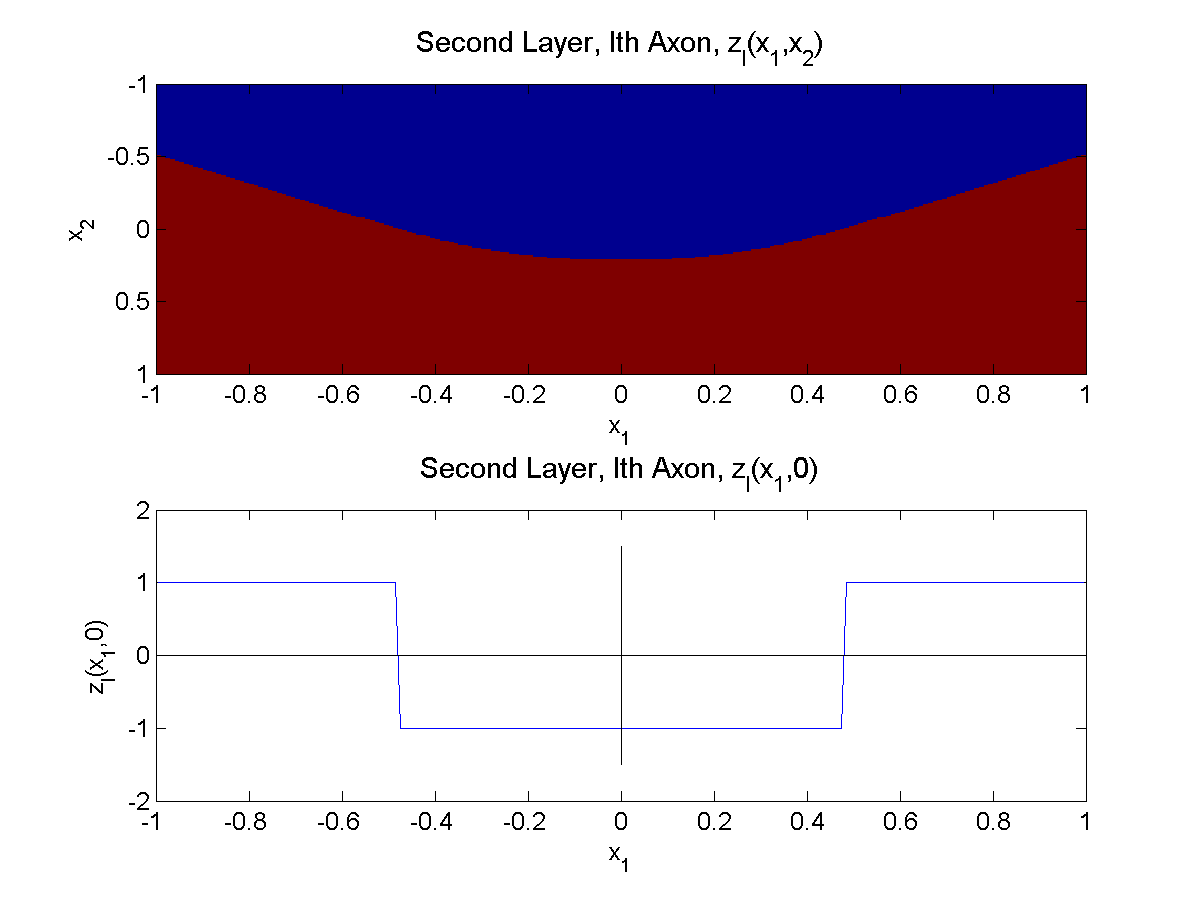
\includegraphics[width=3in]{../lec07/figs/nn_axon2.png}}
\end{frame}

\begin{frame}
  \frametitle{A classifier neural network}
  We can discretize the output by simply using an output nonlinearity,
  e.g., $\hat{y}_k=g(e_k^{(2)})$, for some nonlinearity $g(x)$:
  \begin{small}      \begin{center}
        \tikzstyle{pre}=[<-,shorten <=1pt,>=stealth',semithick,draw=blue]
        \tikzstyle{post}=[->,shorten >=1pt,>=stealth',semithick,draw=blue]
        \begin{tikzpicture}[
            hoop/.style={circle,thick, draw=blue, text=black, fill=orange!35!white, text centered, text width=0.25cm},
            open/.style={circle,thick, draw=blue, text=black, text centered, text width=0.25cm}
          ]
          \node (x0) at (0,0) {$1$};
          \node[open] (x1) at (1,0) {$x_1$};
          \node[open] (x2) at (2,0) {$x_2$};
          \node (x3) at (3,0) {\ldots};
          \node[open] (xp) at (4,0) {$x_D$};
          \node (input) at (7,0) {$\vec{x}$ is the input vector};
          \node (e1sum) at (7,0.75) {$e_k^{(1)} = b_{k}^{(1)}+\sum_{j=1}^Dw_{kj}^{(1)}x_j$};
          %\node (e1vec) at (9,0.75) {$\vec{e}^{(1)}=W^{(1)}\vec{x}+\vec{b}^{(1)}$};
          \node (h0) at (0,1.5) {$1$};
          \node[hoop] (h1) at (1,1.5) {$h_1$} edge[pre](x0) edge[pre](x1) edge[pre](xp);
          \node[hoop] (h2) at (2,1.5) {$h_2$} edge[pre](x0) edge[pre](x1) edge[pre](xp);
          \node (y3) at (3,1.5) {\ldots};
          \node[hoop] (hq) at (4,1.5) {$h_N$} edge[pre](x0) edge[pre](x1) edge[pre](xp);
          \node (hsum) at (7,1.5) {$h_k=\sigma(e_k^{(1)})$};
          %\node (hvec) at (9,1.5) {$\vec{h}=f(\vec{e}^{(1)})$};
          \node (e2sum) at (7,2.25) {$e_k^{(2)}=b_{k}^{(2)}+\sum_{j=1}^N w_{kj}^{(2)}h_j$};
          %\node (e2vec) at (9,2.25) {$\vec{e}^{(2)}=W^{(2)}\vec{h}+\vec{b}^{(2)}$};
          \node[hoop] (y1) at (1,3) {$\hat{y}_1$} edge[pre](h0) edge[pre](h1) edge[pre](hq);
          \node[hoop] (y2) at (2,3) {$\hat{y}_2$} edge[pre](h0) edge[pre](h1) edge[pre](hq);
          \node (y3) at (3,3) {\ldots};
          \node[hoop] (yr) at (4,3) {$\hat{y}_K$} edge[pre](h0) edge[pre](h1) edge[pre](hq);
          \node (ysum) at (7,3) {$\hat{y}_k=g(e_k^{(2)})$};
          %\node (yvec) at (9,3) {$\hat{y}=\vec{e}^{(2)}$};
          \node (zeta1) at (1,3.75) {} edge[pre](y1);
          \node (zeta2) at (2,3.75) {} edge[pre](y2);
          \node (zetar) at (4,3.75) {} edge[pre](yr);
          \node (output) at (2.5,4) {$\hat{y}=h(\vec{x},W^{(1)},\vec{b}^{(1)},W^{(2)},\vec{b}^{(2)})$};
        \end{tikzpicture}
      \end{center}
\end{small}
\end{frame}

\begin{frame}
  \frametitle{Nonlinearities for classifier neural networks}

  \begin{itemize}
  \item {\bf During testing:} the output is passed through a hard
    nonlinearity, e.g., a unit step or a signum.
  \item {\bf During training:} the output is passed through the corresponding soft
    nonlinearity, e.g., sigmoid or tanh.
  \end{itemize}
\end{frame}

\begin{frame}
  \frametitle{Excitation, First Layer: $e_k^{(1)}=b_{k}^{(1)}+\sum_{j=1}^2 w_{kj}^{(1)}x_j$}
  \centerline{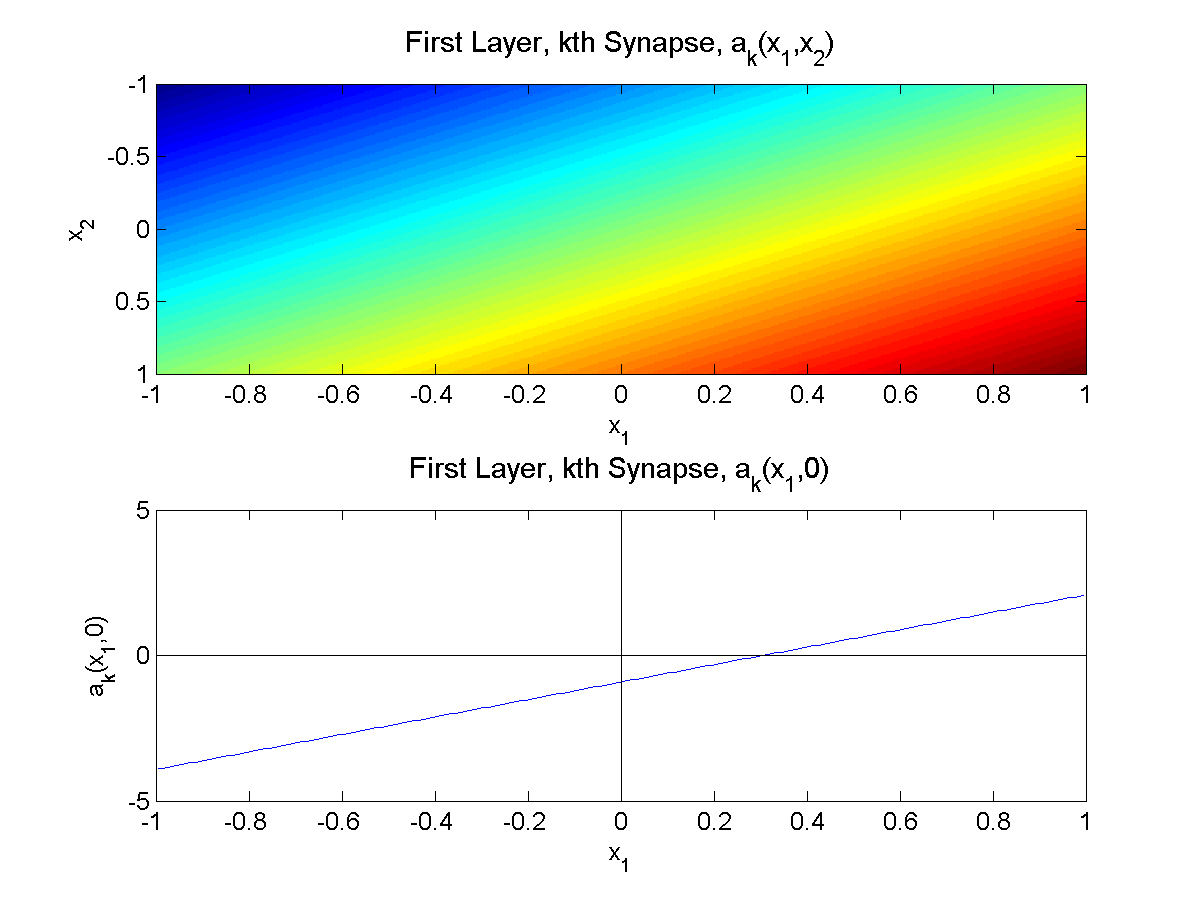
\includegraphics[width=3in]{../lec07/figs/nn_synapse1.png}}
\end{frame}

\begin{frame}
  \frametitle{Activation, First Layer: $h_k=\mbox{tanh}(e_k^{(1)})$}

  Here, I'm using tanh as the nonlinearity for the hidden layer.  But
  it often works better if we use ReLU or PReLU.
  
  \centerline{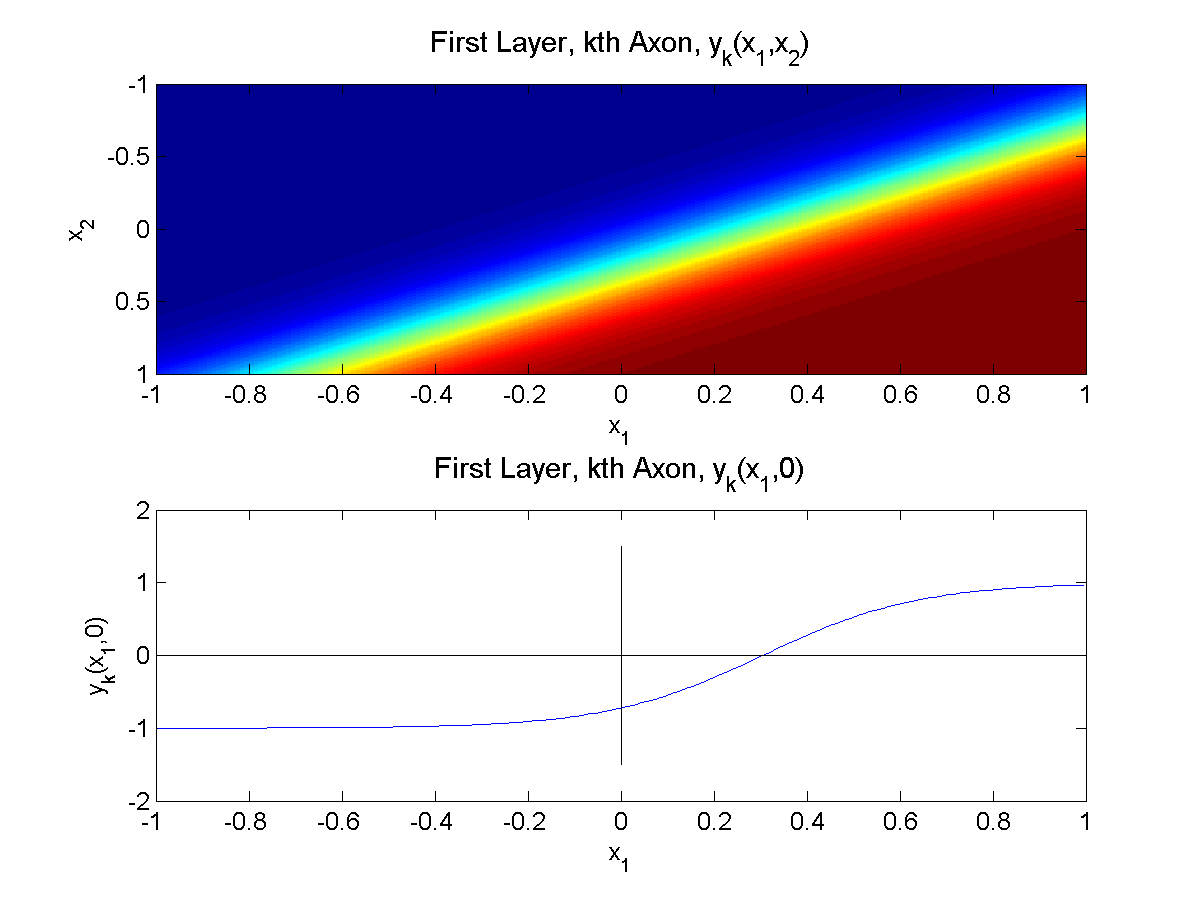
\includegraphics[width=3in]{../lec07/figs/nn_axon1.png}}
\end{frame}

\begin{frame}
  \frametitle{Excitation, Second Layer: $e_k^{(2)}=b_{k}^{(2)}+\sum_{j=1}^2w_{kj}^{(2)}h_j$}
  \centerline{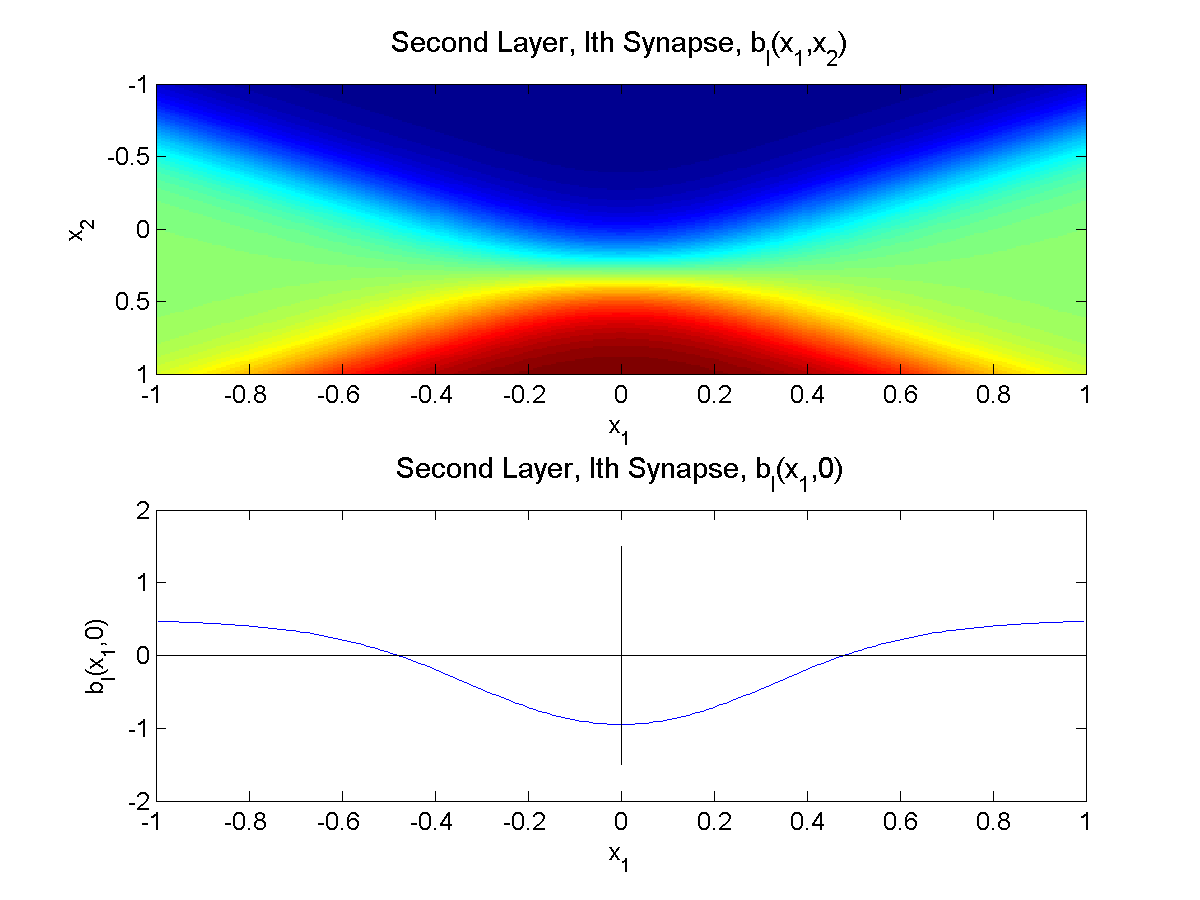
\includegraphics[width=3in]{../lec07/figs/nn_synapse2.png}}
\end{frame}

\begin{frame}
  \frametitle{Activation, Second Layer: $\hat{y}_k=\mbox{sign}(e_k^{(2)})$}

  During  training, the output layer uses  a soft nonlinearity.  During testing, though, the
  soft nonlinearity is replaced with a hard nonlinearity, e.g., signum:
  \centerline{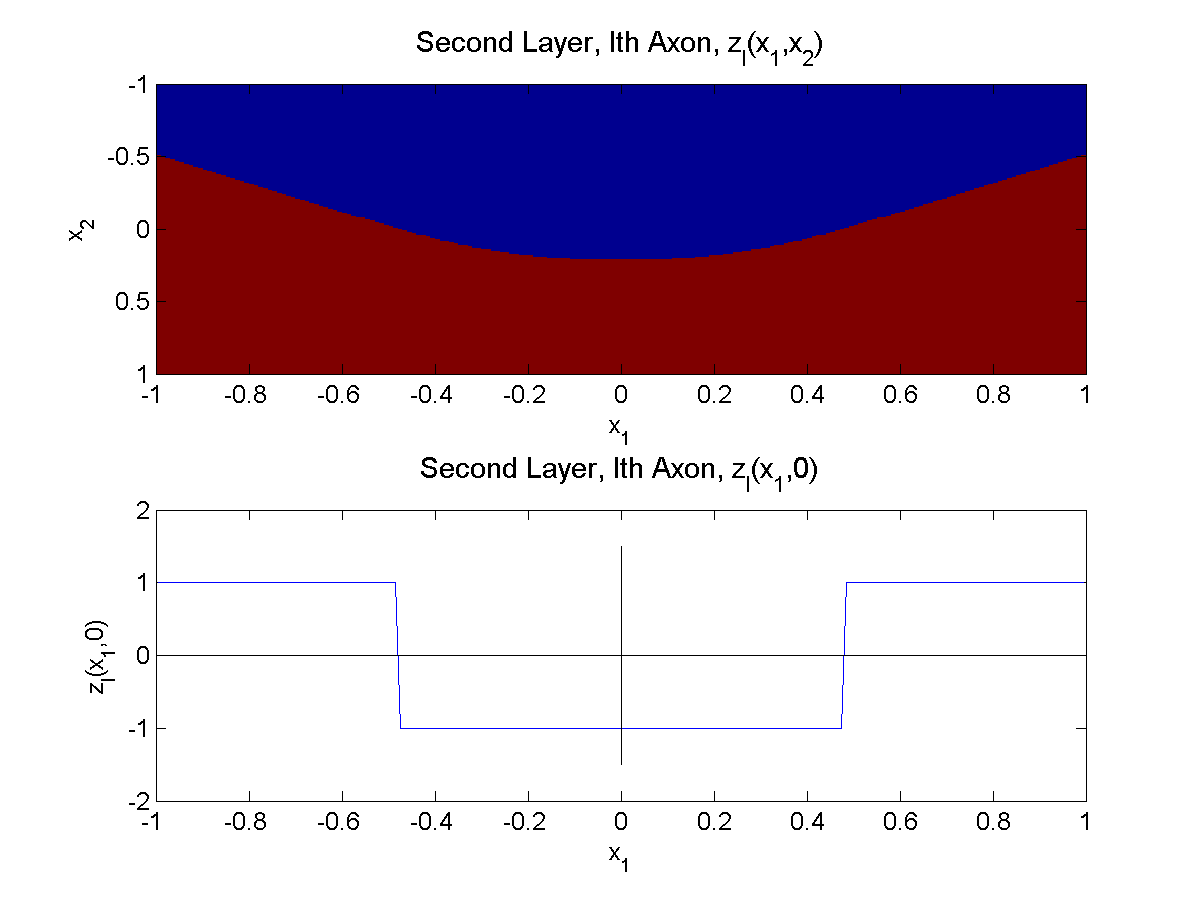
\includegraphics[width=3in]{../lec07/figs/nn_axon2.png}}
\end{frame}

%%%%%%%%%%%%%%%%%%%%%%%%%%%%%%%%%%%%%%%%%%%%%%
\section[BCE Loss]{Binary Cross Entropy  Loss}
\setcounter{subsection}{1}

\begin{frame}
  \frametitle{Review: MSE}
  
  Until now, we've assumed that the loss function is MSE:
  \[{\mathcal L} = \frac{1}{2n}\sum_{i=1}^n\Vert\vec{y}_{i}-\hat{y}(\vec{x}_i)\Vert^2 \]
  \begin{itemize}
  \item MSE makes sense if $\vec{y}$ and $\hat{y}$ are both
    real-valued vectors, and we want to compute
    $\hat{y}_{MMSE}(\vec{x})=E\left[\vec{y}|\vec{x}\right]$.  But
    what if $\hat{y}$ and $\vec{y}$ are discrete-valued (i.e.,
    classifiers?)
  \item Surprise: MSE works surprisingly well, even with
    discrete $\vec{y}$!
  \item But a different metric, binary cross-entropy (BCE) works
    slightly better.
  \end{itemize}
\end{frame}

\begin{frame}
  \frametitle{MSE with a binary target vector}
  \begin{itemize}
  \item Suppose $y$ is just a scalar binary classifier label,
    $y\in\left\{0,1\right\}$ (for example: ``is it a dog or a cat?'')
  \item Suppose that the input vector, $\vec{x}$, is not quite enough
    information to tell us what $y$ should be.  Instead, $\vec{x}$ only tells us
    the probability of $y=1$:
    \[
    y=\left\{\begin{array}{ll}
    1 & \mbox{with probability}~p_{Y|\vec{X}}\left(1|\vec{x}\right)\\
    0 & \mbox{with probability}~p_{Y|\vec{X}}\left(0|\vec{x}\right)
    \end{array}\right.
    \]
  \item In the limit as $n\rightarrow\infty$, assuming that the
    gradient descent finds the global optimum, the MMSE solution gives
    us:
    \begin{align*}
      \hat{y}(\vec{x}) &\rightarrow_{n\rightarrow\infty}  E\left[y|\vec{x}\right]\\
      &= \left(1\times p_{Y|\vec{X}}\left(1|\vec{x}\right)\right) +
      \left(0\times p_{Y|\vec{X}}\left(0|\vec{x}\right)\right)\\
      &= p_{Y|\vec{X}}\left(1|\vec{x}\right)
    \end{align*}
  \end{itemize}
\end{frame}

\begin{frame}
  \frametitle{Pros and Cons of MMSE for Binary Classifiers}

  \begin{itemize}
  \item {\bf Pro:} In the limit as $n\rightarrow\infty$, the global optimum is
    $\hat{y}(\vec{x})\rightarrow p_{Y|\vec{X}}\left(1|\vec{x}\right)$.
  \item {\bf Con:} The sigmoid nonlinearity is hard to train using
    MMSE.  Remember the vanishing gradient problem: $\sigma'(wx)\rightarrow 0$
    as $w\rightarrow\infty$, so after a few epochs of training,
    the neural net just stops learning.
  \item {\bf Solution:} Can we devise a different loss function (not
    MMSE) that will give us the same solution
    ($\hat{y}(\vec{x})\rightarrow p_{Y|\vec{X}}\left(1|\vec{x}\right)$), but
    without suffering from the vanishing gradient problem?
  \end{itemize}
\end{frame}

\begin{frame}
  \frametitle{Binary Cross Entropy}

  Suppose we treat the neural net output as a noisy
  estimator, $\hat{p}_{Y|\vec{X}}(y|\vec{x})$, of the unknown true pmf
  $p_{Y|\vec{X}}\left(y|\vec{x}\right)$:
  \[
  \hat{y}_i = \hat{p}_{Y|\vec{X}}(1|\vec{x}),
  \]
  so that
  \begin{displaymath}
    \hat{p}_{Y|\vec{X}}(y_i|\vec{x}_i)
    =\begin{cases}\hat{y}_i & y_i=1\\1-\hat{y}_i & y_i=0\end{cases}
  \end{displaymath}
  The binary cross-entropy loss is the negative log probability of the
  training data, assuming i.i.d. training examples:
  \begin{align*}
    {\mathcal L}_{BCE} &= -\frac{1}{n}\sum_{i=1}^n \ln\hat{p}_{Y|\vec{X}}(y_i|\vec{x}_i)\\
    &= -\frac{1}{n}\sum_{i=1}^n
    y_i\left(\ln\hat{y}_i\right)+
    (1-y_i)\left(\ln(1-\hat{y}_i)\right)
  \end{align*}
\end{frame}

\begin{frame}
  \frametitle{The Derivative of BCE}

  BCE is useful because it has the same solution as MSE, without
  allowing the sigmoid to suffer from vanishing gradients.  Suppose
  $\hat{y}_i=\sigma(wh_i)$.
  \begin{align*}
    \nabla_w{\mathcal L}
    &=
    -\frac{1}{n}
    \left(
    \sum_{i:y_i=1}\nabla_w\ln\sigma(wh_i)
    +\sum_{i:y_i=0}\nabla_w\ln(1-\sigma(wh_i))
    \right)\\
    &=
    -\frac{1}{n}
    \left(
    \sum_{i:y_i=1}\frac{\nabla_w\sigma(wh_i)}{\sigma(wh_i)}
    +\sum_{i:y_i=0}\frac{\nabla_w(1-\sigma(wh_i))}{1-\sigma(wh_i)}
    \right)\\
    &=
    -\frac{1}{n}
    \left(
    \sum_{i:y_i=1}\frac{\hat{y}_i(1-\hat{y}_i)h_i}{\hat{y}_i}
    +\sum_{i:y_i=0}\frac{-\hat{y}_i(1-\hat{y}_i)h_i}{1-\hat{y}_i}
    \right)\\
    &=
    -\frac{1}{n}\sum_{i=1}^n
    \left(y_i-\hat{y}_i\right)h_i
  \end{align*}
\end{frame}

\begin{frame}
  \frametitle{Why Cross-Entropy is Useful for Machine Learning}
  Binary cross-entropy is useful for machine learning  because:
  \begin{enumerate}
  \item {\bf Just like MSE, it estimates the true class probability:}
    in the limit as $n\rightarrow\infty$, $\nabla_W{\mathcal
      L}\rightarrow E\left[(Y-\hat{Y})H\right]$, which is zero
    only if
    \[
    \hat{Y}=E\left[Y|\vec{X}\right]=p_{Y|\vec{X}}(1|\vec{x})
    \]
  \item {\bf Unlike MSE, it does not suffer from the vanishing
    gradient problem of the sigmoid.}
  \end{enumerate}
\end{frame}
\begin{frame}
  \frametitle{Unlike MSE, BCE does not suffer from the vanishing
    gradient problem of the sigmoid.}
  The vanishing gradient problem
  was caused by
  $\sigma'=\sigma(1-\sigma)$, which
  goes to zero when its input is either plus or minus infinity.
  \begin{itemize}
  \item If $y_i=1$, then differentiating $\ln\sigma$
    cancels the $\sigma$ term in the numerator, leaving only the
    $(1-\sigma)$ term, which is large if and only if the neural net
    is wrong.
  \item If $y_i=0$, then differentiating $\ln(1-\sigma)$
    cancels the $(1-\sigma)$ term in the numerator, leaving only the
    $\sigma$ term, which is large if and only if the neural net is wrong.
  \end{itemize}
  So binary cross-entropy ignores training tokens only if the neural
  net guesses them right.  If it guesses wrong, then
  back-propagation happens.
\end{frame}

%%%%%%%%%%%%%%%%%%%%%%%%%%%%%%%%%%%%%%%%%%%%%%
\section[CE Loss]{Multinomial Classifier: Cross-Entropy  Loss}
\setcounter{subsection}{1}

\begin{frame}
  \frametitle{Multinomial Classifier}

  Suppose, instead of just a 2-class classifier, we want the neural
  network to classify $\vec{x}$ as being one of $K$ different classes.
  There are many ways to encode this, but one of the best is
  \begin{displaymath}
    \vec{y}=\left[\begin{array}{c}y_1\\y_2\\\vdots\\y_K\end{array}\right],~~~
    y_k=\begin{cases}1&k=k^*~~(k~\mbox{is the correct class})\\0&\mbox{otherwise}\end{cases}
  \end{displaymath}
  A vector $\vec{y}$ like this is called a ``one-hot vector,'' because
  it is a binary vector in which only one of the elements is nonzero (``hot'').
  This is useful  because minimizing the MSE loss gives:
  \begin{displaymath}
    \hat{y}=\left[\begin{array}{c}\hat{y}_1\\\hat{y}_2\\\vdots\\\hat{y}_K\end{array}\right]
    =\left[\begin{array}{c}
        \hat{p}_{Y_1|\vec{X}}(1|\vec{x})\\
        \hat{p}_{Y_2|\vec{X}}(1|\vec{x})\\
        \vdots\\
        \hat{p}_{Y_K|\vec{X}}(1|\vec{x})
        \end{array}\right],
  \end{displaymath}
  where the global optimum of
  $\hat{p}_{Y_k|\vec{X}}(y|\vec{x})\rightarrow
  p_{Y_k|\vec{X}}(y|\vec{x})$ as $n\rightarrow\infty$.
\end{frame}

\begin{frame}
  \frametitle{One-hot vectors and Cross-entropy loss}
  
  The cross-entropy loss, for a training database coded with one-hot vectors, is
  \begin{align*}
    {\mathcal L}_{CE} &=-\frac{1}{n}\sum_{i=1}^n\sum_{k=1}^K y_{ki}\ln\hat{y}_{ki}
  \end{align*}
  This is useful because:
  \begin{enumerate}
  \item {\bf Like MSE, Cross-Entropy has an asymptotic global optimum at:}
    $\hat{y}_k\rightarrow p_{Y_k|\vec{X}}(1|\vec{x})$.
  \item {\bf Unlike MSE, Cross-Entropy with a softmax nonlinearity
    suffers no vanishing gradient problem.}
  \end{enumerate}
\end{frame}

\begin{frame}
  \frametitle{Softmax Nonlinearity}

  The multinomial cross-entropy loss is only well-defined if
  $0<\hat{y}_{ki}<1$, and it is only well-interpretable if
  $\sum_k\hat{y}_{ki}=1$.  We can guarantee these two properties by
  setting
  \begin{align*}
    \hat{y}_k &= \softmax_k\left(W\vec{h}\right)\\
    &= \frac{\exp(\bar{w}_k\vec{h})}{\sum_{\ell=1}^K
      \exp(\bar{w}_\ell\vec{h})},
  \end{align*}
  where $\bar{w}_k$ is the $k^{\textrm{th}}$ row of the $W$ matrix.
\end{frame}

\begin{frame}
  \frametitle{Sigmoid is a special case of Softmax!}

  \begin{displaymath}
    \softmax_k\left(W\vec{h}\right)
    = \frac{\exp(\bar{w}_k\vec{h})}{\sum_{\ell=1}^K
      \exp(\bar{w}_\ell\vec{h})}.
  \end{displaymath}
  Notice that, in the 2-class case, the softmax is just exactly a
  logistic sigmoid function:
  \begin{displaymath}
    \softmax_1(W\vec{h}) = \frac{e^{\bar{w}_1\vec{h}}}{e^{\bar{w}_1\vec{h}}+e^{\bar{w}_2\vec{h}}}
    = \frac{1}{1+e^{-(\bar{w}_1-\bar{w}_2)\vec{h}}}  =\sigma\left((\bar{w}_1-\bar{w}_2)\vec{h}\right)
  \end{displaymath}
  so everything that you've already learned about the sigmoid applies
  equally well here.
\end{frame}

%%%%%%%%%%%%%%%%%%%%%%%%%%%%%%%%%%%%%%%%%%%%%%%%%%%%%%%%%%%%%%%%%%%%%%
\section{Summary}
\setcounter{subsection}{1}

\begin{frame}
  \frametitle{Nonlinearities Summarized}
  \begin{itemize}
  \item Unit-step and signum nonlinearities, on the hidden layer,
    cause the neural net to compute a piece-wise constant approximation
    of the target function. Unfortunately, they're not differentiable, so they're not
    trainable.
  \item Sigmoid and tanh are differentiable approximations of
    unit-step and signum, respectively.  Unfortunately, they suffer
    from a vanishing gradient problem: as the weight matrix gets
    larger, the derivatives of sigmoid and tanh go to zero, so error
    doesn't get back-propagated through the nonlinearity any more.
  \item ReLU has the nice property that the output is a
    piece-wise-linear approximation of the target function, instead of
    piece-wise constant.  It also has no vanishing gradient problem.
    Instead, it has the dying-ReLU problem.
  \item Softplus, Leaky ReLU, and PReLU are different solutions to the
    dying-ReLU problem.
  \end{itemize}
\end{frame}

\begin{frame}
  \frametitle{Error Metrics Summarized}
  \begin{itemize}
    \item Use MSE to achieve $\hat{y}\rightarrow
      E\left[\vec{y}|\vec{x}\right]$.  That's almost always what you
      want.
    \item For a binary classifier with a sigmoid output, BCE loss gives you
      the MSE result without the vanishing gradient problem.
    \item For a multi-class classifier with a softmax output, CE loss gives you
      the MSE result without the vanishing gradient problem.
    \item After you're done training, you can make your cell phone app
      more efficient by throwing away the uncertainty:
      \begin{itemize}
      \item Replace softmax output nodes with max
      \item Replace logistic output nodes with unit-step
      \item Replace tanh output nodes with signum
      \end{itemize}
  \end{itemize}
\end{frame}



\end{document}

